% Options for packages loaded elsewhere
\PassOptionsToPackage{unicode,linktoc=all,pdfwindowui,pdfpagemode=FullScreen,pdfauthor=``Anna
Cristina de Araújo Rodrigues'',pdftitle=``Naufrágio e resurreição da
imagem'',pdfproducer =``ABNT-Quarto''}{hyperref}
\PassOptionsToPackage{hyphens}{url}
%
\documentclass[
  letterpaper,
  a4paper,
  12pt]{scrbook}

\usepackage{amsmath,amssymb}
\usepackage{lmodern}
\usepackage{iftex}
\ifPDFTeX
  \usepackage[T1]{fontenc}
  \usepackage[utf8]{inputenc}
  \usepackage{textcomp} % provide euro and other symbols
\else % if luatex or xetex
  \usepackage{unicode-math}
  \defaultfontfeatures{Scale=MatchLowercase}
  \defaultfontfeatures[\rmfamily]{Ligatures=TeX,Scale=1}
  \setmainfont[]{ETbb}
  \setsansfont[Scale=MatchUppercase]{TeX Gyre Heros}
\fi
% Use upquote if available, for straight quotes in verbatim environments
\IfFileExists{upquote.sty}{\usepackage{upquote}}{}
\IfFileExists{microtype.sty}{% use microtype if available
  \usepackage[]{microtype}
  \UseMicrotypeSet[protrusion]{basicmath} % disable protrusion for tt fonts
}{}
\makeatletter
\@ifundefined{KOMAClassName}{% if non-KOMA class
  \IfFileExists{parskip.sty}{%
    \usepackage{parskip}
  }{% else
    \setlength{\parindent}{0pt}
    \setlength{\parskip}{6pt plus 2pt minus 1pt}}
}{% if KOMA class
  \KOMAoptions{parskip=half}}
\makeatother
\usepackage{xcolor}
\usepackage[top=30mm,left=30mm,right=20mm,bottom=20mm,footskip=10mm,twoside,a4paper]{geometry}
\usepackage[normalem]{ulem}
\setlength{\emergencystretch}{3em} % prevent overfull lines
\setcounter{secnumdepth}{5}
% Make \paragraph and \subparagraph free-standing
\ifx\paragraph\undefined\else
  \let\oldparagraph\paragraph
  \renewcommand{\paragraph}[1]{\oldparagraph{#1}\mbox{}}
\fi
\ifx\subparagraph\undefined\else
  \let\oldsubparagraph\subparagraph
  \renewcommand{\subparagraph}[1]{\oldsubparagraph{#1}\mbox{}}
\fi


\providecommand{\tightlist}{%
  \setlength{\itemsep}{0pt}\setlength{\parskip}{0pt}}\usepackage{longtable,booktabs,array}
\usepackage{calc} % for calculating minipage widths
% Correct order of tables after \paragraph or \subparagraph
\usepackage{etoolbox}
\makeatletter
\patchcmd\longtable{\par}{\if@noskipsec\mbox{}\fi\par}{}{}
\makeatother
% Allow footnotes in longtable head/foot
\IfFileExists{footnotehyper.sty}{\usepackage{footnotehyper}}{\usepackage{footnote}}
\makesavenoteenv{longtable}
\usepackage{graphicx}
\makeatletter
\def\maxwidth{\ifdim\Gin@nat@width>\linewidth\linewidth\else\Gin@nat@width\fi}
\def\maxheight{\ifdim\Gin@nat@height>\textheight\textheight\else\Gin@nat@height\fi}
\makeatother
% Scale images if necessary, so that they will not overflow the page
% margins by default, and it is still possible to overwrite the defaults
% using explicit options in \includegraphics[width, height, ...]{}
\setkeys{Gin}{width=\maxwidth,height=\maxheight,keepaspectratio}
% Set default figure placement to htbp
\makeatletter
\def\fps@figure{htbp}
\makeatother


\usepackage{expl3}              % Usado pelo estilo citação abnt-ibid
\expandafter\def\csname ver@l3regex.sty\endcsname{} 
\usepackage{lastpage}           % Usado pela Ficha catalográfica
\usepackage{indentfirst}        % Indenta o primeiro parágrafo de cada seção.
\usepackage{nomencl}            % Necessário para o commando makeindex
\usepackage{pdfpages}  
\usepackage[
    automark,
    autooneside=false,% <- if you want to use \leftmark and \rightmark in a one sided document
    headsepline=false
  ]{scrlayer-scrpage} % Usado para modificar o cabeçalho
\usepackage[hang,flushmargin]{footmisc}

\usepackage{etoolbox}
\usepackage[hyphens,spaces,obeyspaces]{xurl}
\usepackage{ragged2e}
\usepackage[onehalfspacing]{setspace}
\setkomafont{pageheadfoot}{ \textsc}
\graphicspath{{imgs/}} % diretório de imagens
\renewenvironment{quote}
  {\par\singlespacing\small\list{}{\rightmargin=0cm \leftmargin=4cm }%
   \item\relax}
  {\endlist}
\makeatletter
\makeatother
\makeatletter
\@ifpackageloaded{bookmark}{}{\usepackage{bookmark}}
\makeatother
\makeatletter
\@ifpackageloaded{caption}{}{\usepackage{caption}}
\AtBeginDocument{%
\ifdefined\contentsname
  \renewcommand*\contentsname{Índice}
\else
  \newcommand\contentsname{Índice}
\fi
\ifdefined\listfigurename
  \renewcommand*\listfigurename{Lista de Figuras}
\else
  \newcommand\listfigurename{Lista de Figuras}
\fi
\ifdefined\listtablename
  \renewcommand*\listtablename{Lista de Tabelas}
\else
  \newcommand\listtablename{Lista de Tabelas}
\fi
\ifdefined\figurename
  \renewcommand*\figurename{Figura}
\else
  \newcommand\figurename{Figura}
\fi
\ifdefined\tablename
  \renewcommand*\tablename{Tabela}
\else
  \newcommand\tablename{Tabela}
\fi
}
\@ifpackageloaded{float}{}{\usepackage{float}}
\floatstyle{ruled}
\@ifundefined{c@chapter}{\newfloat{codelisting}{h}{lop}}{\newfloat{codelisting}{h}{lop}[chapter]}
\floatname{codelisting}{Listagem}
\newcommand*\listoflistings{\listof{codelisting}{Lista de Listagens}}
\makeatother
\makeatletter
\@ifpackageloaded{caption}{}{\usepackage{caption}}
\@ifpackageloaded{subcaption}{}{\usepackage{subcaption}}
\makeatother
\makeatletter
\@ifpackageloaded{tcolorbox}{}{\usepackage[many]{tcolorbox}}
\makeatother
\makeatletter
\@ifundefined{shadecolor}{\definecolor{shadecolor}{rgb}{.97, .97, .97}}
\makeatother
\makeatletter
\makeatother
\ifLuaTeX
\usepackage[bidi=basic]{babel}
\else
\usepackage[bidi=default]{babel}
\fi
\babelprovide[main,import]{brazilian}
% get rid of language-specific shorthands (see #6817):
\let\LanguageShortHands\languageshorthands
\def\languageshorthands#1{}
\ifLuaTeX
  \usepackage{selnolig}  % disable illegal ligatures
\fi
\usepackage[style=abnt,]{biblatex}
\addbibresource{references.bib}
\IfFileExists{bookmark.sty}{\usepackage{bookmark}}{\usepackage{hyperref}}
\IfFileExists{xurl.sty}{\usepackage{xurl}}{} % add URL line breaks if available
\urlstyle{same} % disable monospaced font for URLs
\hypersetup{
  pdftitle={Naufrágio e resurreição da imagem},
  pdfauthor={Anna Cristina de Araújo Rodrigues},
  pdflang={pt-BR},
  hidelinks,
  pdfcreator={LaTeX via pandoc}}

\title{Naufrágio e resurreição da imagem}
\usepackage{etoolbox}
\makeatletter
\providecommand{\subtitle}[1]{% add subtitle to \maketitle
  \apptocmd{\@title}{\par {\large #1 \par}}{}{}
}
\makeatother
\subtitle{a fotografia de Aylan Kurdi inquieta o imaginário
contemporâneo}
\author{Anna Cristina de Araújo Rodrigues}
\date{}

\begin{document}
\frontmatter
\maketitle

\frontmatter
\frenchspacing
\onehalfspacing
% \RaggedRight


%  Cabeçalho, rodapé, seção, capítulo e paginação

\makeatletter
\apptocmd{\@part}{\parttitle{#2}}{}{}
\def\parttitle#1{\gdef\theparttitle{#1}}
\def\theparttitle{} % initialization
\makeatother

\renewcommand{\sectionmark}[1]{\markright{\spacedlowsmallcaps{#1}}}

\pagestyle{scrheadings}
\clearscrheadfoot
\automark[section]{chapter}
\ohead*{\pagemark}
\ofoot{\Ifthispageodd{\leftmark}{\rightmark}}
% \ifoot[\theparttitle]{\theparttitle}




% 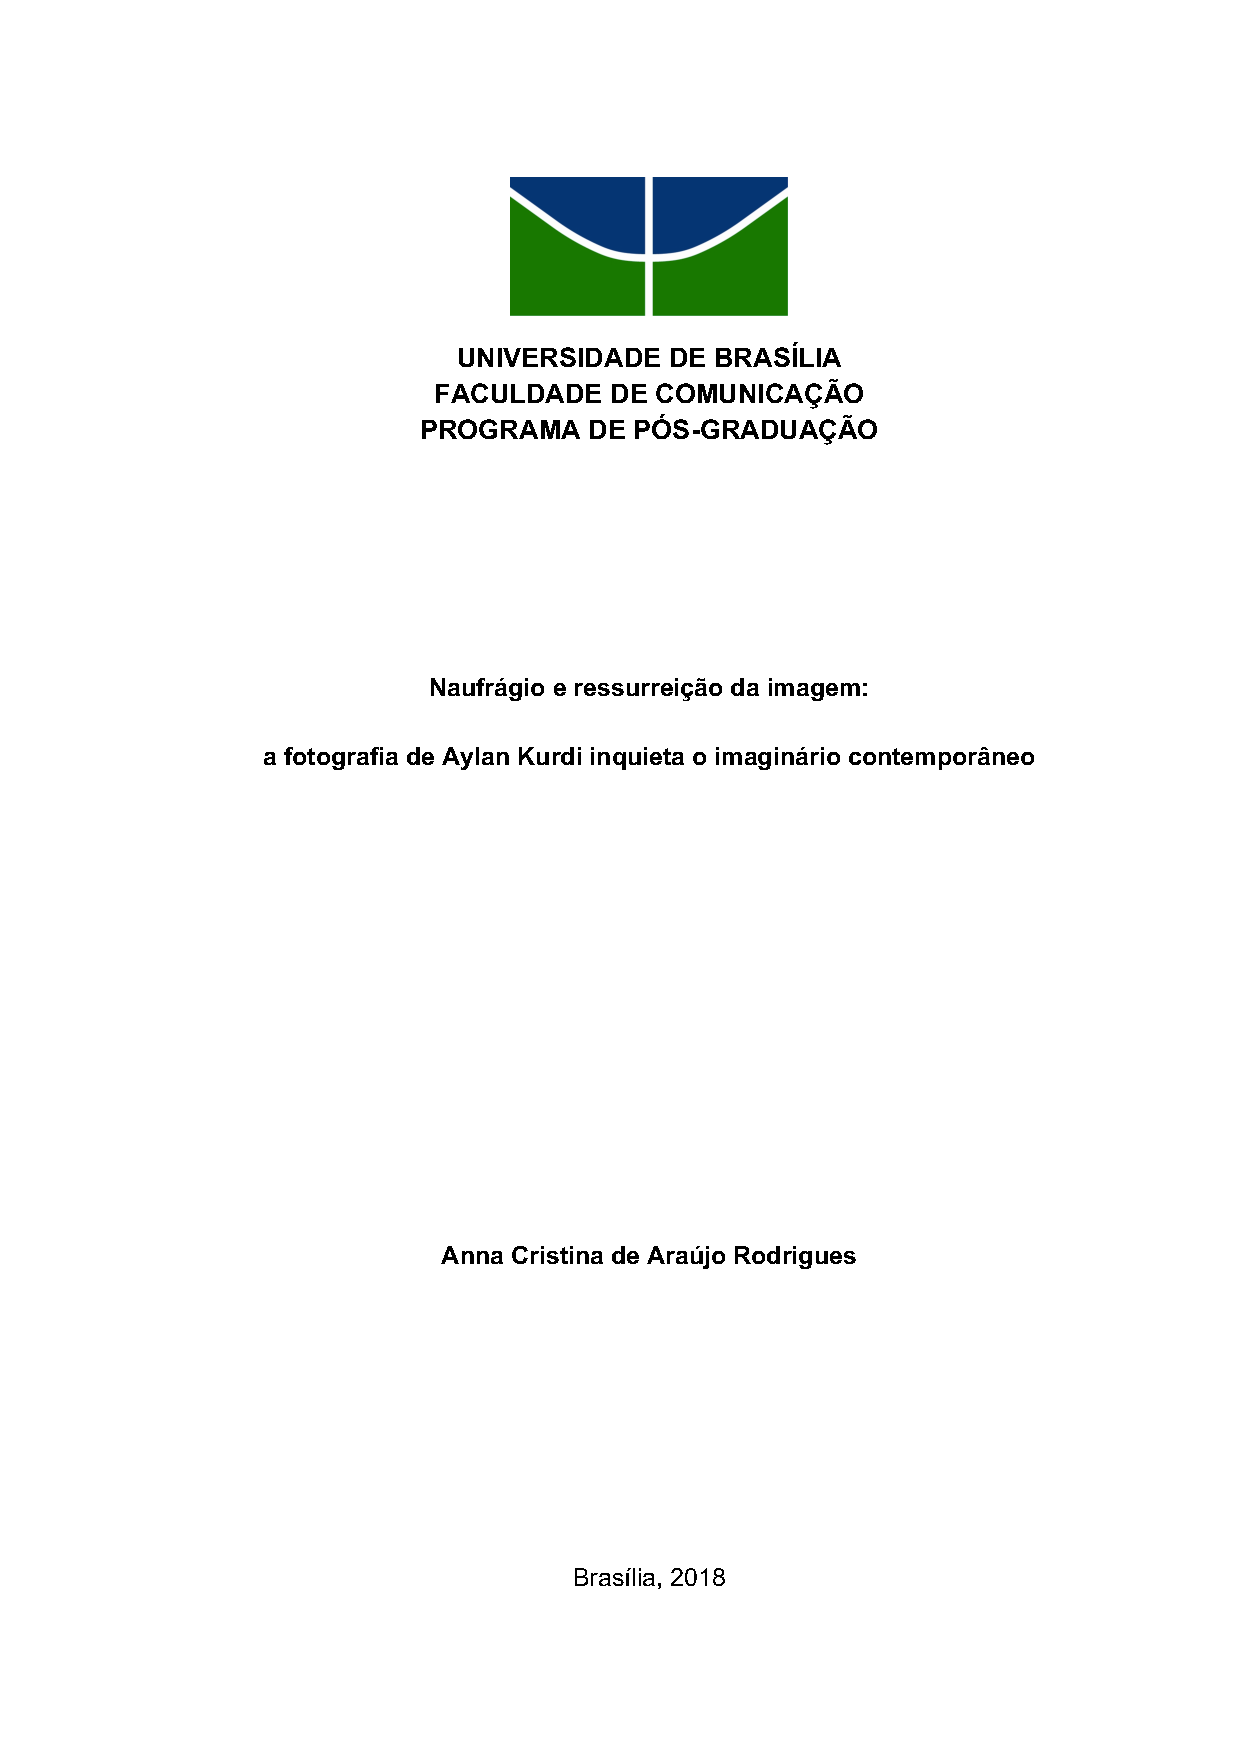
\includepdf{imgs/capa.pdf}
% \pagebreak
% 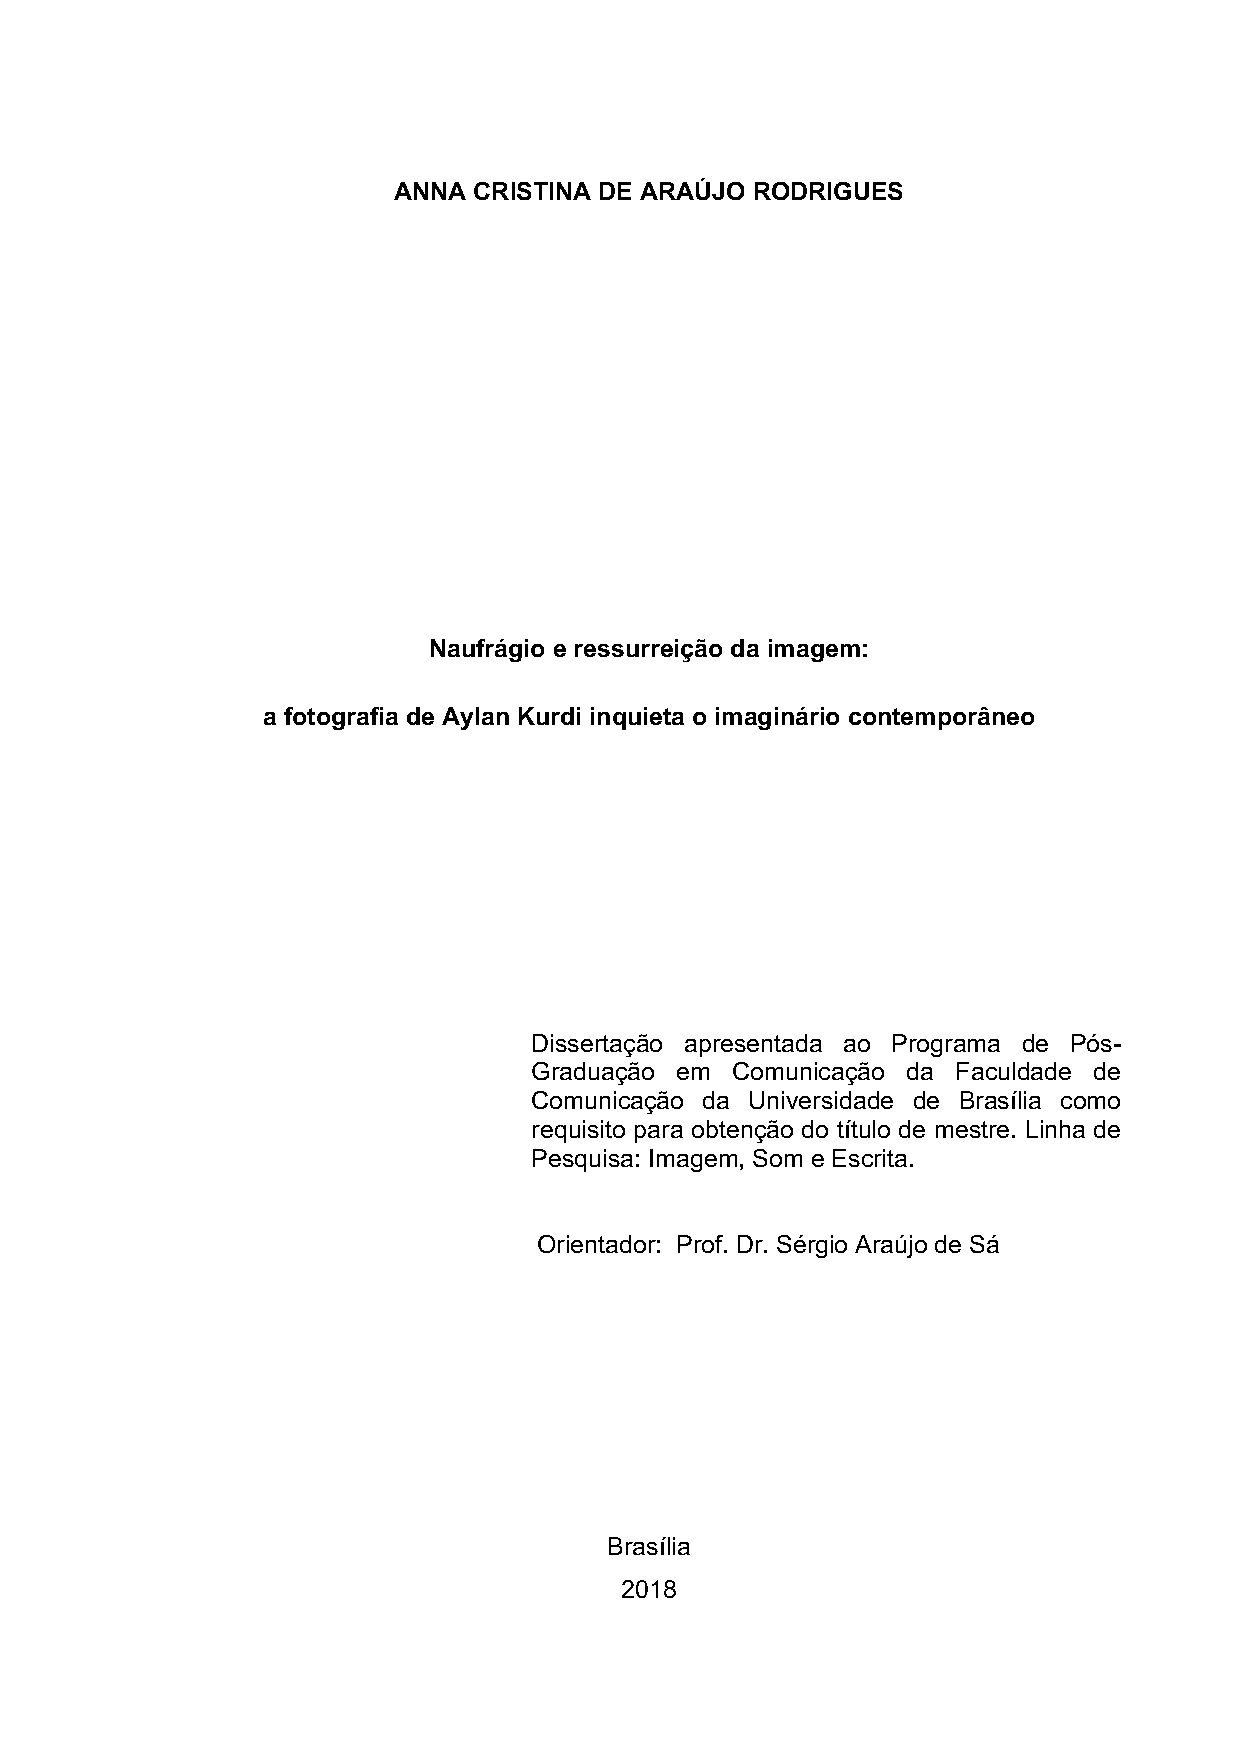
\includepdf{imgs/folha_de_rosto.pdf}
% \pagebreak
% 
\includepdf{imgs/ficha_catalografica.pdf}
% \author{$author$}
% \title{$title$}
% \def\degreetitle{$degreetype$}
% \degrees{$degrees$}
% \def\affiliation{$affiliation$}

% % Add subject and keywords below
% \hypersetup{
%      %pdfsubject={The Subject},
%      %pdfkeywords={Some Keywords},
%      pdfauthor={$author$},
%      pdftitle={$title$},
%      pdfproducer={Quarto with LaTeX}
% }



% \titulo{Modelo Canônico de\\ Trabalho Acadêmico com \abnTeX}
% \autor{Equipe \abnTeX}
% \local{Brasil}
% \data{2014, v-1.9.2}
% \orientador{Lauro César Araujo}
% \coorientador{Equipe \abnTeX}
% \instituicao{%
%   Universidade do Brasil -- UBr
%   \par
%   Faculdade de Arquitetura da Informação
%   \par
%   Programa de Pós-Graduação}
% \tipotrabalho{Tese (Doutorado)}
% % O preambulo deve conter o tipo do trabalho, o objetivo, 
% % o nome da instituição e a área de concentração 
% \preambulo{Modelo canônico de trabalho monográfico acadêmico em conformidade com
% as normas ABNT apresentado à comunidade de usuários \LaTeX.}

\ifdefined\Shaded\renewenvironment{Shaded}{\begin{tcolorbox}[frame hidden, enhanced, borderline west={3pt}{0pt}{shadecolor}, breakable, boxrule=0pt, sharp corners, interior hidden]}{\end{tcolorbox}}\fi

\renewcommand*\contentsname{Sumário}
{
\setcounter{tocdepth}{2}
\tableofcontents
}
\listoffigures
\listoftables
\mainmatter
\bookmarksetup{startatroot}

\hypertarget{copyright-notice}{%
\chapter*{Copyright notice}\label{copyright-notice}}
\addcontentsline{toc}{chapter}{Copyright notice}

\markboth{Copyright notice}{Copyright notice}

\bookmarksetup{startatroot}

\hypertarget{introduuxe7uxe3o}{%
\chapter{Introdução}\label{introduuxe7uxe3o}}

A questão central do projeto de pesquisa que~deu origem ao presente
estudo, desenvolvido no Programa de Pós-Graduação em Comunicação --
Mestrado, na linha de pesquisa Imagem, Som e Escrita,~refere-se à
fotografia de Aylan Kurdi, menino sírio de 3 anos de idade, encontrado
morto em uma praia da Turquia no dia 2 de setembro de 2015, em
decorrência da fuga malfadada de sua família em busca de se salvar da
guerra civil que assola a Síria desde 2011.

Depois de um pedido de asilo negado pelo governo do Canadá, a família
Kurdi resolveu atravessar o~Mediterrâneo em um barco inflável com
destino à Europa;~o barco naufragou na costa turca;~três membros dessa
família~morreram~-- entre eles, Aylan; Nilüfer Demir, fotógrafa da
agência Dogan, capturou a imagem de Aylan morto na praia; e a foto foi
distribuída pela Reuters Ancara/DHA ainda em 2 de setembro de 2015.

Essa~fotografia~alcançou~a primeira página de diversos jornais do mundo
inteiro e milhões de usuários de redes sociais;~despertou a indignação
da audiência; transformou-se em símbolo da atual crise de refugiados;~e
se desdobrou em dezenas de~imagens nascidas no seio de um movimento
social~digital~que trouxe para a discussão~a empatia de que ainda somos
capazes, a despeito do individualismo\footnote{O conceito de
  individualismo aqui utilizado é o descrito por Giles Lipovetsky,
  sobretudo em seu livro \emph{A era do vazio -- ensaios sobre o
  individualismo contemporâneo} (edição de 2005, publicada no Brasil
  pela Editora Manole). Para compreendê-lo, é preciso estar ciente de
  que o filósofo francês associa individualismo com consumo e liberdade
  como forma de alcançar a realização pessoal, mas também com solidão e
  dificuldade de comunicação. Essa combinação gera uma cultura
  paradoxal: descentrada e heteróclita, materialista e psi, pornô e
  discreta, inovadora e retrô, consumista e ecologista, sofisticada e
  espontânea, espetacular e criativa. ``Na sociedade individualista de
  hoje -- especialmente na sociedade de consumo --, os indivíduos não
  são mais obrigados a se integrar dentro do grupo. Portanto, é
  inevitável que sintam solidão, uma vez que carregam o fardo de ter que
  construir suas próprias vidas. Quanto mais liberdade temos para
  construir nossas vidas, mais fraco é o elo social. Não é de se admirar
  que hoje em dia muitas pessoas se sintam diferentes, não como os
  demais. Isso é uma das marcas registradas do individualismo.
  {[}...{]}. (Lipovetsky em entrevista em 15.05.2017, disponível em:
  \textless https://www.fronteiras.com/entrevistas/gilles-lipovetsky-a-politica-agora-e-tida-como-profissao-nao-existem-mais-estadistas\textgreater.
  Acesso em: 27 jan. 2018.} tão característico da contemporaneidade.

O~poder da imagem de veicular experiências coletivas é, como se observa,
assunto importante~desta dissertação.~Consideramos a ideia de que as
imagens de Aylan Kurdi~que integram este trabalho, a partir da
divulgação da fotografia~que chocou o mundo, são expressões de um
comprometimento coletivo com a causa dos refugiados.~São a prova da
possibilidade de reação contra o individualismo,~ainda que transitória e
apesar de os tempos que correm serem hiperindividualistas. É isso que
tantos ecos da fotografia de~Nilüfer Demir~estão nos dizendo.

Antes, porém, de partir para discussões sobre os impactos da fotografia
de Aylan Kurdi sobre diferentes setores da sociedade, vamos nos deter em
conceitos fundamentais para compreensão do objeto da pesquisa, como
imagem e imaginário. A pergunta inicial que nos fizemos, então, foi:~o
que é uma imagem?

Para~\textcite{joly2012introducao}:

\begin{quote}
{[}...{]}~parece que imagem pode ser tudo e seu contrário -- visual e
imaterial, fabricada e~``natural'', real e virtual, móvel e imóvel,
sagrada e profana, antiga e contemporânea, vinculada à vida e à morte,
analógica, comparativa, convencional, expressiva, comunicativa,
construtora e destrutiva, benéfica e ameaçadora.
\autocite[pp.27]{joly2012introducao}~
\end{quote}

De fato, usamos a palavra~``imagem'' para designar objetos~imaginários
ou concretos.~No capítulo 1, discutiremos o conceito de imagem e
buscaremos estender esse conceito tanto quanto possível, de forma a
alcançar~categorias que organizam o que chamamos de imagens, por
exemplo:~imagens~fixas~(ou estáticas) e imagens~em movimento;~imagens
visuais, mentais e de síntese;~imagens tradicionais e
imagens~técnicas~--~essas~últimas terão~especial destaque já~que
trataremos, sobretudo, de fotografia, que é a imagem técnica por
excelência e o processo que permitiu a reprodução de imagens por meio de
um aparelho, alterando profundamente nosso modo de enxergar e conhecer o
mundo, quiçá de viver. Passaremos pelas funções sociais das imagens,
preparando o terreno para chegar a um ponto central do estudo:~a
fotografia~de Aylan Kurdi mostrou ao mundo a morte dessa criança e, em
troca, deu-lhe notoriedade, transformando-a~em símbolo de uma crise
humanitária de consequências muito graves.~

As imagens~sempre cumpriram o desejo humano de representar a realidade.
Mas fazem mais que isso:~veiculam conteúdos subjacentes, imersos em um
campo de nosso ser -- o imaginário -- à espera do momento em que poderão
vir à tona, trazendo consigo~um conhecimento que é, ao mesmo tempo,
individual e coletivo, mas muitas vezes com particularidades que só os
artistas logram alcançar. No capítulo 2, trataremos~do imaginário com
vistas a buscar nesse campo do saber elementos capazes de explicar~de
que maneira é possível compreender as imagens artísticas inspiradas na
fotografia em estudo desde setembro de 2015, nos mais variados lugares
do mundo -- ilustrações, grafites, murais,~esculturas~e~performances.~A
morte de Aylan Kurdi trouxe~consigo, entre outras, uma imagem que habita
o imaginário ocidental há séculos: o naufrágio. Nossa história
trágico-marítima é muito antiga -- tem origem em relatos bíblicos, com a
Arca de Noé;~passa pela Idade Média, período do qual destacaremos um dos
episódios mais instigantes do imaginário ocidental, que é a Cruzada das
Crianças,~com base no~Prêmio Nobel de Literatura Mario Vargas Llosa, que
recria~a fábula misturando história e ficção; atravessa os séculos XV,
XVI e chega~ao século XVII, período que ficou conhecido como o das
grandes navegações ou a era dos descobrimentos;~e chega aos dias de
hoje, em que o mundo inteiro aguarda, ansiosamente, a explicação do
sumiço de um submarino argentino desaparecido~desde o dia 15 de novembro
de 2017~e que reuniu os países mais poderosos do mundo em torno da
decifração do que ocorreu de fato com a embarcação e seus 44
tripulantes.~Nesse segundo capítulo, evocaremos ainda personagens que
transitam nesse contexto~trágico-catastrófico, incluindo Nilüfer Demir,
a fotógrafa que se notabilizou por decidir tornar a tragédia de Aylan
conhecida, Magnus Wennman, cujas fotografias resultaram na exposição
\emph{Where the children sleep}, sobre crianças refugiadas no Oriente
Médio e na Europa, e outros responsáveis por fotografias
icônicas,\footnote{Neste estudo, utilizamos o termo ``icônico/icônica''
  para identificar fotografias que se tornaram famosas e foram/são
  usadas como símbolo.} mundialmente conhecidas e tornadas históricas
graças ao seu poder transformador. Discutiremos esse suposto estatuto
transformador a partir de questões como:~por que não se sai ileso depois
de ver a fotografia de Aylan Kurdi e que poder tem~essa fotografia a
ponto de inquietar o mundo inteiro, alterando as eleições canadenses,
expondo as mazelas da política da União Europeia para refugiados,
estimulando uma empatia que conseguiu arrecadar fundos para atender,
especificamente, refugiados sírios e elevando o tema da crise migratória
e dos refugiados a um dos assuntos mais discutidos e destacados de 2015?
Passaremos pelo seu poder de persuasão,~mais uma vez~sob a
influência~de~Mario Vargas Llosa, considerando aspectos observáveis na
fotografia de Aylan, que é jornalística, mas que desliza para o campo
ficcional e põe em xeque a fronteira entre o real e o ficcional.~

O personagem central deste trabalho, como se pode observar, é Aylan
Kurdi --~o herói trágico,~segundo~a classificação de~Aristóteles,~em
sua~\emph{Poética}, pois que é alguém cuja desgraça não foi provocada
pelo vício ou por degeneração de caráter de qualquer espécie, mas pelo
destino. No capítulo 3, trataremos desse destino -- a guerra que matou
Aylan Kurdi --~e do~caráter pós-moderno que envolve a discussão de
conceitos que geraram muita confusão nos últimos tempos -- em especial,
``refugiados'' e ``migrantes''. Discutiremos também~as demonstrações de
empatia observadas em decorrência da repercussão da fotografia~de~Aylan
e a divergência na visão de autores que se debruçaram sobre esse aspecto
especificamente.~

A rapidez~-- menos de 24 horas -- e o alcance~dos~eventos~que envolveram
a morte de Aylan Kurdi~foram possíveis porque vivemos em uma época e em
uma sociedade em que as tecnologias digitais\footnote{CEALE.
  \emph{Tecnologia digital}. Disponível em:
  \textless http://www.ceale.fae.ufmg.br/app/webroot/glossarioceale/verbetes/tecnologia-digital\textgreater.
  Acesso em: 31 jul. 2017.}~criam condições para que os indivíduos atuem
ativamente na propagação~de informações, inclusive, produzindo seus
próprios conteúdos e os distribuindo.~O~advento da internet e das redes
sociais permitiu o surgimento de uma forma de comunicação que continua a
ser de massa, porque alcança audiência global, mas é autocomunicação
(CASTELLS, 2015), na medida em que~muitos se comunicam com muitos. A
espinha dorsal dessa comunicação é~a rede~de computadores, a linguagem
empregada é digital, e os emissores/receptores são globalmente
distribuídos e estão em permanente conectividade. No capítulo 4, nos
ocuparemos dessa~revolução tecnológica~que~deu suporte a uma incrível
ampliação da atuação de indivíduos e grupos sociais, mas destacaremos
que~a evolução cultural das sociedades é mais ampla do que o
desenvolvimento de tecnologias~-- a~tecnologia é apenas um aspecto
material de uma evolução cultural que,~a partir do final dos anos 1970,
se configurou como época em que se observou uma reorganização profunda
do funcionamento social e cultural das sociedades democráticas
avançadas, marcada por rápida expansão do consumo, intensificação~da
comunicação de massa, fortalecimento do individualismo e do hedonismo e
perda da fé no futuro revolucionário~\autocite{lipovetsky2004tempos}.~

Nesse contexto, à comunicação cabe um papel~fundamental, bem distinto
das práticas de 40 anos atrás. As redes digitais de comunicação deram
origem a novas relações de poder, hoje determinadas pelos atuais
processos e formas da comunicação socializada que ampliam a autonomia
dos sujeitos comunicantes em relação às corporações de comunicação, de
modo que os clássicos e estanques papéis de emissor e receptor cedem
lugar a sujeitos que são tanto emissores quanto receptores de mensagens,
ao mesmo tempo.~Como tal, desafiam o poder do Estado e de organizações
da sociedade, uma vez que, historicamente, o exercício da autoridade
sempre dependeu do controle da informação e da comunicação.~As
consequências disso são relevantes e se desdobram em reações e opiniões
divergentes. Por exemplo, segundo~Umberto~Eco:

\begin{quote}
As mídias sociais deram o direito à fala a legiões de imbecis que,
anteriormente, falavam só no bar, depois de uma taça de vinho, sem
causar dano à coletividade. Diziam imediatamente a eles para calar a
boca, enquanto agora eles têm o mesmo direito à fala que um ganhador do
Prêmio Nobel. (ECO, 2015 apud~ÉPOCA, 2016)~\autocite[apud][]{epoca2016}
\end{quote}

Da mesma forma que a imbecilidade ganha voz, a sensatez e a lucidez
encontram seu espaço. O filósofo francês Gilles~Lipovetsky
\autocite*{lipovetsky2004tempos} nos lembra que não é justo que sejamos
reduzidos a seres hiperconsumidores, porque a vida não é só consumo.
Ainda somos empáticos, nos indignamos com as injustiças, defendemos o
meio ambiente e os direitos humanos: ``Não perdemos nossa alma: o
decadentismo moral é um mito''
\autocite[pp.~413]{lipovetsky2004tempos}~Os tempos hipermodernos
descritos por \autocite{lipovetsky2004tempos} supervalorizam o
individualismo, o que não impede ações como a demonstração de
resistência dada por artistas do mundo inteiro que, ao produzir
ilustrações, esculturas, grafites,~murais e performances, tornaram menos
efêmera a imagem de Aylan Kurdi. Suas manifestações visuais tiveram o
claro objetivo de impedir, em alguma medida, que a fotografia de Nilüfer
Demir~caísse~no circuito do tempo real, tão característico do
jornalismo. O que eles fizeram foi um movimento contrário a essa
lógica,~utilizando, para isso, a imagem, em ação de ``produções
artísticas orientadas pela livre exploração e transgressão da
tecnologia'' \autocite[ p.~13]{hora2015},~à maneira do que
\textcites{sa2007}[ p.~17]{sa2007} observa a respeito do escritor:
``Escritor não é repórter''. Sua ação está pautada no ``desejo de dar
durabilidade ao que é passageiro e fugaz {[}...{]}''.

Nesse contexto, é preciso entender que ``{[}...{]} a informação
conforma, dá forma à socialização contemporânea. Esta não se dá mais por
tradição, religião ou moral, mas sim pela `ação da informação mediática
e das imagens'\,'' (SÁ, 2010, p.~16).

Para nos aprofundarmos nos conteúdos a que nos propusemos em cada
capítulo, utilizamos bibliografia dedicada a compreender a fotografia e
outras imagens que se enquadram no conceito de \textcite{aumont2011}
~adotado neste trabalho~e buscamos respostas também em autores que se
ocuparam de estudar o imaginário, esse campo do saber~que
constitui~``uma via de acesso para as verdades indemonstráveis: a
existência da alma, o além, a morte, os mistérios do amor... Ali onde a
dialética bloqueada não consegue penetrar, a imagem mítica fala
diretamente à alma''~\autocite[ p.17]{durand1996}.

Não poderíamos~ignorar~que~as~imagens com as quais estamos lidando são
difundidas pela mídia, por isso~``encontram-se onipresentes em todos os
níveis de representação e da psique do homem ocidental ou
ocidentalizado'' \autocite[ p.~32]{durand1996}. Essas imagens midiáticas
nos acompanham permanentemente e é mais que necessário compreender seu
papel como fenômeno fundamental de nossa sociedade e~a revolução
cultural que seu surgimento implicou. Para isso, nos apoiaremos em
Castells e~em~sua teoria do poder da comunicação, como caminho
para~apreender a sociedade em rede e suas novas formas de organização
econômica, social, política,~cultural~e tecnológica.~

O papel da fotografia na~comunicação~não é assunto novo,
mas~esta~pesquisa procura ir além dessa discussão, já que o mundo
hiperconsumista, hipertecnicizado e hiperconectado transformou
indelevelmente a forma como nos comunicamos, aumentando a influência da
sociedade civil e dos atores sociopolíticos não institucionais em
diversos setores da vida em sociedade.~Como já adiantado, a~ampliação da
habilidade de atores individuais de se manifestar sobre todos os temas
de interesse para a humanidade passa pela evolução tecnológica dos
últimos 40 anos, mas, conforme Castells (2015, p.~34), ``nenhuma
tecnologia determina coisa alguma, uma vez que processos sociais estão
incorporados em um conjunto complexo de relações sociais''.

Nesse sentido, tentar compreender um fenômeno midiático como a
superexposição das imagens de Aylan Kurdi, considerando esse conjunto
complexo de relações, é uma forma não exatamente nova de pensar~a
comunicação, mas certamente bastante atual de abordá-la. O fato
de~artistas~reagirem à imagem fotográfica, produzindo mais e mais
imagens~e distribuindo-as para o mundo inteiro via internet é,~também,
um fenômeno típico dos tempos que correm:~

\begin{quote}
{[}...{]}~o capitalismo artista não criou apenas um novo modo de
produção, mas favoreceu, com a cultura democrática, o advento de uma
sociedade e de um indivíduo estético ou, mais exatamente, transestético
por não depender mais do esteticismo à moda antiga, compartimentado e
hierarquizado.~\autocite[ p.30-31]{lipovetsky2004tempos}~
\end{quote}

O interesse deste estudo recai, portanto, menos nas questões históricas
e políticas da cobertura jornalística do drama dos refugiados do que em
seus aspectos culturais marcadamente~contemporâneos. É nesse sentido que
este estudo se enquadra na linha de pesquisa Imagem, Som e Escrita do
Programa de Pós-Graduação em Comunicação da Faculdade de Comunicação da
Universidade de Brasília, ``direcionada para as discussões teóricas e
pontuais sobre imagem, som e escrita em suas relações com as práticas
sociais e experiências dos sujeitos na contemporaneidade''.\footnote{Disponível
  em:
  \textless http://fac.unb.br/pos-graduacao/209-imagem-e-som\textgreater.
  Acesso em: 12 jan. 2017.}

Esta~pesquisa~foi feita~a partir de uma abordagem~qualitativa~na medida
em que optamos por~trabalhar numa perspectiva exploratória, de natureza
básica, cujo objetivo é~investigar um fenômeno comunicacional que se
materializou, primeiro, numa fotografia, depois, em representações
secundárias da imagem~de Aylan Kurdi, e essas
imagens~foram~divulgadas~insistentemente~via redes sociais digitais.

O procedimento técnico~baseou-se~em pesquisa bibliográfica (livros,
artigos jornalísticos e científicos, dissertações e teses etc.) e
documental -- as~fotografias~e demais expressões artísticas que as fotos
inspiraram. E a pesquisa pretendeu construir um conhecimento teórico,
propriamente científico, já que o que está sendo proposto é responder à
questão de~\emph{por que é}, a partir da investigação
das~\emph{causas}~e dos \emph{princípios} do fenômeno, o que nos leva ao
objetivo~central da pesquisa, que poderíamos resumir em:~investigar~a
imagem~visual~como objeto criado pelas pessoas e acrescentado ao mundo
pela atividade humana e que serve para representá-lo, como forma de
reconhecer sua importância fundamental para a sociedade e as formas de
comunicação~contemporâneas.

As fotos feitas por~Nilüfer~Demir e as ilustrações obtidas no
rastreamento da \emph{hashtag}{[}\^{}5{]}
\#kiyiyavuraninsanlik{[}\^{}6{]} constituem, portanto, o \emph{corpus}
da pesquisa, assim como imagens de esculturas, murais, performances~e
exposição de arte que derivaram da fotografia.~

A análise de dados qualitativos é etapa que exige atenção, tempo e
perspicácia do pesquisador. Para~\textcite{minayo2008}, há obstáculos
que devem ser superados, por exemplo, a ilusão da transparência. Isso
significa que os dados coletados não revelam com transparência o real.
Logo, não se deve fazer uma interpretação espontânea e literal deles,
pois são sempre registros simbólicos e polissêmicos:

\begin{quote}
É no campo da subjetividade e do simbolismo que se afirma a abordagem
qualitativa. {[}...{]} A abordagem qualitativa realiza uma aproximação
fundamental e de intimidade entre sujeito e objeto, uma vez que ambos
são da mesma natureza: ela se volve com empatia aos motivos, às
intenções, aos projetos dos atores, a partir dos quais as ações, as
estruturas e as relações tornam-se significativas. \autocite[
p.244]{Minayo1993}
\end{quote}

É nesse sentido que os estudos sobre o imaginário serão de grande
importância. Refletir sobre o imaginário nos leva a tomar consciência do
que subjaz à organização das imagens responsáveis por estruturar nosso
modo de ver a vida e o mundo, de observar, pensar sentir e comunicar.
Sendo o imaginário um mundo de símbolos, é ali que residem mitos e
arquétipos que dão forma ao ser que somos e em que podemos nos
transformar.~Então, é ali que buscaremos as simbologias e polissemias do
real que se nos apresenta.

No contexto desta pesquisa, esse real é a vida/morte de Aylan Kurdi,
traduzida em imagens midiáticas que apontam para um poder
``primordialmente exercido pela construção de significado na mente
humana por meio de processos de comunicação postos em prática nas redes
multimídia de comunicação de massa locais e globais {[}...{]}''
\autocite[ p.471]{castells2015}. Ou seja, um poder que habita nosso
imaginário individual e coletivo e que pode ser outro, a depender do
modo como nos comunicamos.~

Por fim, práticas de comunicação~se dividem em~interpessoal e mediada.
Em termos sociais, a comunicação mediada~terá, aqui, maior destaque por
constituir o ambiente simbólico~em que~recebemos, processamos~e
enviamos~as mensagens que produzem sentido em nossa vida e conformam a
cultura. Nesse processo, encontram-se as chances de modificar, em favor
de indivíduos e grupos,~as relações de poder~em operação.~

\bookmarksetup{startatroot}

\hypertarget{sobre-a-imagem...}{%
\chapter{Sobre a imagem...}\label{sobre-a-imagem...}}

\hypertarget{considerauxe7uxf5es-iniciais}{%
\section{Considerações iniciais}\label{considerauxe7uxf5es-iniciais}}

As imagens são o produto e o reflexo histórico da civilização. Não
surgiram com a internet, ou com a TV, nem mesmo com o cinema e~a
fotografia. Muito antes de todas essas tecnologias audiovisuais que
comumente associamos à veiculação de imagens, as pessoas já~pintavam
quadros, desenhavam em diversos tipos de suportes, produziam gravuras.

No paleolítico,~registraram aspectos da vida, utilizando desenhos
rupestres, estatuetas, pinturas e desenhos. E essas imagens tinham
objetivo -- talvez fazer algum tipo de comunicação.~Dois milhões e meio
de anos nos separam~desses tempos que hoje são evocados como o início da
história da arte, embora o conceito de arte tal como compreendemos hoje
não se ajuste perfeitamente a essas imagens. De lá para cá, a imagem vem
servindo a diferentes propósitos humanos, anteriores, inclusive, à
própria~arte.~

Na Antiguidade romana, o termo~``imagem'' referia-se à máscara mortuária
usada em funerais, o que indica que essa palavra remetia~à~morte e ao
culto dos mortos. No Egito Antigo, a imagem tinha objetivos políticos e
religiosos. No Renascimento, a separação~entre representação religiosa~e
representação profana deu origem a imagens pictóricas, o que significa
que só recentemente, em termos históricos, passamos a produzir imagens
também para nos referirmos ao mundo que não tem relação apenas com a
religião.

Atualmente, a imagem tanto pode servir a todos os propósitos políticos e
religiosos de então, como também a estéticos, artísticos e científicos.
Na medicina, por exemplo, os exames de imagem, como tomografias
computadorizadas e ressonâncias magnéticas,{[}\^{}7{]}~são largamente
usados para diagnosticar diversas doenças. E há todo um setor~produtivo
que se ocupa exclusivamente de desenvolver essas tecnologias para
aplicação na saúde.~

Até aqui, tratamos da imagem visual: representação gráfica, plástica ou
fotográfica. Mas há outros tipos de imagem, por exemplo, a imagem
mental. Embora não seja essa imagem o objeto central de estudo a que nos
propusemos,~é preciso citá-la para diferenciar os tipos de imagens
com~os quais lidamos ao longo da vida e para já prepararmos o campo
para~adentrar o imaginário, tema com que também trabalharemos nesta
dissertação.~

``A imagem mental corresponde~à impressão que temos, quando, por
exemplo, lemos ou ouvimos a descrição de um lugar, de~\emph{vê-lo~}quase
como se estivéssemos lá'' \autocite[ p.~19]{joly2012introducao}. Não
entraremos na discussão sobre a (in)existência de tais imagens.~Diremos
apenas que há quem defenda que não passam de descrições verbais e
abstratas, cujo significado não pode ser apreendido senão pela
linguagem. Isso porque seu caráter subjetivo torna-a inacessível a
outros indivíduos, além de quem imagina.~Nessa categoria, incluem-se os
sonhos, por exemplo.

Em algumas áreas do conhecimento, estudar imagem significa fazer
associações mentais sistemáticas para melhor~compreender um ser ou um
objeto, uma profissão, uma prática humana. Assim, os estudiosos buscam
compreender a ``imagem da mulher'' em dado contexto sociocultural, ou a
imagem de uma empresa, de um grupo político ou religioso. E nos estudos
da língua, o objeto é a imagem verbal, mais comumente a metáfora.~

Além das imagens visuais e mentais, há as imagens de síntese, que são
aquelas produzidas por computador para criar universos virtuais, como os
videogames, que tiveram início com imagens grosseiras e evoluíram para
as atuais imagens interativas que perturbam a distinção entre o real e o
virtual.

\begin{quote}
``O holograma -- imagem a \emph{laser} em três dimensões -- faz parte
dessas novas imagens desconcertantes, por um lado, por seu aspecto
realista, mas também por seu aspecto fantasmático de duplo perfeito,
flutuante, como em suspensão'' \autocite[ p.27]{joly2012introducao}.
\end{quote}

Um~\emph{show}~em tributo ao cantor Renato Russo tornou-se
histórico~para os brasilienses: na noite do sábado 29 de junho de 2013,
no Estádio~Nacional Mané Garrincha, em Brasília, um holograma recriou em
ambiente digital a sensação de estar diante do artista. ``A imagem de
Renato Russo surge no palco em quatro dimensões. Altura, largura,
profundidade e saudade. E 45 mil pessoas sabiam que ele não estava ali,
e que ele estava~sim''.{[}\^{}8{]}

Como bem descreve \textcite{joly2012introducao}:~

\begin{quote}
Instrumento de comunicação, divindade, a imagem assemelha-se ou
confunde-se com o que representa. Visualmente imitadora, pode enganar ou
educar. Reflexo, pode levar ao conhecimento. A Sobrevivência, o
Sagrado,~a Morte, o Saber, a Verdade, a Arte, se tivermos um mínimo de
memória, são os campos a que o simples termo~``imagem''~nos vincula.
\autocite[ p.19]{joly2012introducao}
\end{quote}

Imagem~é tudo isso e talvez mais, porque não é tão simples classificar~o
que vemos, em que pensamos ou com que sonhamos: seriam imagens todas
elas? Para efeito da identificação do objeto~central desta pesquisa,
adotaremos, então, o conceito de \textcite{aumont2011} , a seguir.

\hypertarget{o-conceito-de-imagem}{%
\section{O conceito~de imagem}\label{o-conceito-de-imagem}}

Para tão diversos empregos~do vocábulo ``imagem'', há de haver um ponto
comum que justifique~significados~diferentes para~um mesmo significante.
Para Joly, esse ponto comum parece ser a analogia: ``Material ou
imaterial, visual ou não, natural ou fabricada, uma `imagem' é antes de
mais nada~\emph{algo que se assemelha a outra coisa}'' \autocite[ p.28
-- grifos da autora]{joly2012introducao}.~

Partindo~para uma delimitação~da~imagem~objeto deste trabalho,
adotaremos o conceito de \textcite{aumont2011}:~

\begin{quote}
A imagem, na nossa cultura, é tudo isso: uma reprodução de um aspecto do
mundo, captada pela sensibilidade mais ou menos individual, mais ou
menos genérica e típica de um mediador (artista ou não), que nos
comunica informações e sentimentos, suscitando em nós outros ainda -- e
é também um objeto novo acrescentado ao mundo, um objeto que vive a sua
vida, tornando-se célebre ou permanecendo ignorado.~\autocite[
p.~7]{aumont2011}~
\end{quote}

As palavras~que completam~o~excerto de \autocite[ p.~7]{aumont2011} são
as seguintes: ``A imagem é um sósia do mundo, mas um sósia deformado,
por muito realista que seja, e~que exerce sobre nós a atração e eficácia
mágicas do duplo, ao mesmo tempo que o encanto próprio de um objeto
puramente visual''.~Com essas palavras, o que percebemos é que~a imagem
é sempre um objeto segundo~(presente)~com relação a outro (ausente)~que
ela representa.~E, ao representar, produz sentido(s) que suscita(m), por
parte de quem a olha, interpretações.~

E chegamos ao que \textcite{joly2012introducao} considera como
consequência da tomada de consciência do estatuto da imagem:

\begin{quote}
{[}...{]} constatar que esse denominador comum da analogia, ou da
semelhança, coloca de imediato a imagem na categoria das
\emph{representações}. Se ela parece é porque~\emph{ela não é a própria
coisa}: sua função é, portanto, evocar, querer dizer outra coisa que não
ela própria, utilizando o processo da semelhança. Se a imagem é
percebida como~\emph{representação}, isso quer dizer que a imagem é
percebida como signo.~\autocite[ p.~39~-- grifos
nossos]{joly2012introducao}~
\end{quote}

Essa é uma perspectiva da teoria semiótica, que propõe considerar a
imagem como signo e que ajuda a compreender o estatuto da imagem. Roland
Barthes, que será aqui citado~algumas~vezes, é referência importante
dessa linha teórica. Isso significa que, embora esta não seja uma
pesquisa de semiótica, a análise das imagens que compõem
o~\emph{corpus}~será feita com o apoio da semiótica.~

Assumir pressupostos semióticos, como perceber a imagem como signo,
representação, exige reflexão sobre~a(s) mensagem(ns)
de~determinada~imagem. Quem produz e expõe uma imagem tem,
certamente,~objetivo(s), tem algo a dizer e não o faz por palavras. Quem
olha uma imagem pode ou não se sentir atraído e, caso seja atraído, pode
se perguntar sobre o conteúdo daquela imagem. Se as representações são
compreendidas pelo indivíduo que olha a imagem, é porque existe, entre
ele e o outro que a produziu, um mínimo de convenção sociocultural que
permitiu a comunicação,~evocando~a semelhança,~o traço e~a convenção,
isto é, o ícone,~o índice~e~o símbolo.~Mas Joly~(2012, p.~42)~nos
alerta: ``Reconhecer motivos nas mensagens visuais e interpretá-los são
duas operações mentais complementares, mesmo que tenhamos a impressão de
que são simultâneas''.~

A experiência de olhar confere importância especial às imagens visuais,
mas, como bem destaca Novaes (2005):~

\begin{quote}
As imagens não são, portanto, apenas, nem mesmo principalmente, um
objeto de contemplação do olho e do espírito. É através delas que o
olhar se realiza em nós com o que nos vem de fora; da mesma maneira que
é através das imagens do espírito que o homem realiza o que está no
mundo. \emph{As imagens permitem, pois, este duplo movimento: sair de si
e trazer o mundo para dentro~de si}. (NOVAES, 2005, p.~10-11 -- grifos
nossos)~
\end{quote}

A vida contemporânea tornou-se muito pródiga na produção e exibição de
imagens. Não há como~parar de consumir imagens, e o tempo da nossa
existência parece insuficiente para a nossa capacidade de pensar
sobre~elas, de compreender o mundo a partir delas.~E imagem sem
pensamento pode ser uma fórmula empobrecedora para a vida do indivíduo e
perigosa para a coletividade, porque reduz a experiência de viver a mera
distração (NOVAES, 2005, p.~14), consequentemente, não conduz a um
universo de luz e sombra, que é o imaginário, onde moram as imagens,~mas
também~a~\uline{fan}tasia, o~\uline{fan}tástico,
o~\uline{fan}tasma~(essas palavras vêm do grego\,\emph{phos}, ``luz'',
do verbo\,\emph{phaínein}, ``fazer aparecer'', pois o que se mostra
iluminado aparece, se faz notar).~

Há, portanto, necessária articulação entre imagens que nos cercam e
ideias já formadas e que constituem o imaginário, e tanto as primeiras
quanto as segundas só podem significar algo se formos capazes de pensar
sobre elas, o que vai além da simples distração de olhar para elas. A
partir desse pensar, chega-se ao deciframento do mundo.~Neste trabalho,
o resultado que se espera é decifrar a fotografia de Aylan Kurdi, em
primeiro lugar, mas também aquelas que surgiram como eco desta, de tal
forma que seja possível observar o duplo movimento descrito por Novaes
(2005) -- o que é ``sair de si'', o que é ``trazer o mundo para dentro
de si'' e como esse vaivém resulta na compreensão de um aspecto do mundo
e da vida.

Imagens têm~extraordinária força de convencimento.~Mostram pela
afirmação porque ignoram a negação;~não explicam, não comparam, não
deduzem~--~tudo o que dizem poderia se resumir em:~aí está,~é
assim.~Tornam presente qualquer passado ou ausência. ``A imagem quer
anular a morte'' (WOLFF, 2005, p.~32).~Por isso, nas sociedades
tradicionais, grande parte das imagens produzidas~é composta de deuses e
de mortos -- imagens sagradas que precederam o nascimento da arte.~

Nas sociedades~modernas -- surgidas a partir do século XVI, na Europa, e
consolidadas no final do século XIX --,~imagens sagradas e
profanas~transbordam. O prodigioso desenvolvimento de técnicas
automáticas de reprodução -- fotografia, cinema, televisão, imagens~de
síntese~-- pôs imagens em todos os lugares, imagens de tudo, de todos e
para todos, num movimento que deu acesso a todos à cultura e à realidade
do mundo~(WOLFF, 2005).

Sobre~``realidade'', porém, é preciso~dizer: na contemporaneidade, ter
acesso ao real via imagens técnicas é uma~ilusão, posto que o que vemos
são recortes, fragmentos: ``Será que imaginamos quantos acontecimentos,
mais graves, mais importantes, históricos, foram omitidos porque não
havia câmera para filmá-los ou porque decidimos~não
os~mostrar?''~(WOLFF, 2005, p.~44). Mais que isso, será que está claro
para o olhar que as imagens técnicas~não são -- como podem parecer -- o
real se reproduzindo sozinho, sem a atuação humana? ~

Segundo Wolff (2005),~

\begin{quote}
O mais perigoso poder da imagem é fazer crer que ela não é uma imagem,
fazer-se esquecer como imagem. Antes da arte, olhávamos o ícone e
acreditávamos ver o próprio deus, diretamente, sem representação. Depois
da arte, olhamos para a televisão e cremos ver a própria realidade,
diretamente, sem representação. A causa está ausente, o trabalho de
produção da imagem não é mais visto na imagem, a imagem não pode ser
vista como imagem. Diante dessas imagens ao vivo e em tempo real,
atravessamos a tela, no real registrado, a representação é negada como
representação {[}...{]}. (WOLFF, 2005, p.~43)~
\end{quote}

A esse propósito, o artista surrealista belga René Magritte inquietou o
mundo com uma obra revolucionária e fundamental que nos faz pensar sobre
a relação que existe entre o objeto em si e sua representação:
\emph{Ceci n'est pas une pipe} (Isto não é um cachimbo), pinturas em que
ele chama a atenção para o fato sempre esquecido de que a pintura de um
cachimbo não é um cachimbo, mas uma pintura. Dois dos quadros dessa
série são os mais conhecidos e os mais importantes: \emph{La trahison
des images}, de 1928, e \emph{Les deux mystères}, de 1966.

{[}{]}{[}17{]}

\protect\hypertarget{_Toc507740886}{}{}\textbf{Figura 1 -- A traição das
imagens}

{[}{]}{[}18{]}

\protect\hypertarget{_Toc507740887}{}{}\textbf{Figura 2 -- Os dois
mistérios}

\begin{quote}
O título ``A traição das imagens'' chama a atenção para a circunstância
de as coisas não serem o que parecem ser e, em particular, para o fato,
que deveria ser óbvio mas não é, de que a representação de uma coisa
nunca será mais do que isto: a representação de uma coisa e não a
própria coisa. Não sabemos como as coisas são em si, apenas como elas
aparecem aos nossos limitados sentidos e à nossa limitada mente em dado
momento limitado. {[}...{]} O título ``Os dois mistérios'' mostra que o
pintor não ficou contente com um mistério ``só'' e resolveu duplicá-lo,
décadas depois do primeiro quadro e de toda a repercussão que ele gerou.
{[}...{]} O primeiro mistério é o da traição das imagens, que são
imagens das coisas e não as próprias coisas que imaginamos. O segundo
mistério é o da explicitação da metaficção, isto é, da ficção dentro da
ficção que, paradoxalmente, tanto revela quanto esconde o labirinto
vertiginoso em que a arte vem nos jogando há tanto tempo.{[}\^{}9{]}
\end{quote}

Neste trabalho,~trataremos de imagens visuais fixas, especificamente de
uma fotografia~jornalística,~e passaremos por manifestações visuais~como
representações secundárias dessa fotografia.~Isso obriga a que abordemos
a imagem analógica sob pontos de vista que~tenham íntima relação com
procedimentos técnicos~de produzir imagens~e~com a condição
interconectada da sociedade em rede e dos meios de comunicação, mas
também sob o ponto de vista dos sentidos que essas imagens adquirem e
das relações que mantêm com ideias guardadas no imaginário. Os sentidos
partirão do real, mas transitarão pelo imaginário e pelo ficcional, na
medida em que nosso objeto de estudo parece se situar nas fronteiras
desses campos, muito mais do que no real que o fotojornalismo sugere.

A fotografia jornalística em questão~foi feita pela fotojornalista
turca~Nilüfer Demir, no dia 2 de setembro de 2015,~em~Bodrum, na
Turquia, em que se vê uma criança morta nas areias da praia -- é Aylan
Kurdi, 3 anos, sírio de origem curda,~muçulmano, provavelmente sunita
(como a maioria dos muçulmanos), que fugia da guerra em seu país e
morreu após o barco em que viajava com a família e mais algumas pessoas
naufragar. E as perguntas que guiaram este estudo foram: por que aquela
foto~-- e não outra -- atraiu~a atenção de jornais de tantos países a
ponto de ser estampada na primeira página, no dia seguinte à morte de
Aylan, 3 de setembro de 2015? O que essa foto trouxe consigo que explica
a reação imediata da audiência e as manifestações visuais de
internautas? ``As imagens fotográficas~não falam~-- se impõem pela
imobilidade e pelo silêncio'', nos ensinou Philippe~Dubois~durante o
curso ``Cinema e fotografia: autobiografia, autorretrato e arte da
memória em Raymond~Depardon,~Agnès~Varda, Chris~Marker~e
Jean~Eustache'', na Universidade de Brasília, em abril de 2017.~``A
própria mudez do que seria, hipoteticamente, compreensível nas fotos é o
que constitui seu caráter atraente e provocador'', nos
ensina~Sontag~(2004, p.~34).~Como compreender o que na imagem
fotográfica atrai e provoca~aqueles que a olham? Por que não saímos
intactos depois de olhar essa foto~e as representações que dela
partiram?

A seguir, as funções da imagem e as relações entre imagem e técnica
serão discutidas para, partindo disso, concluirmos o capítulo com a
fotografia como processo de (re)produção de imagens.~

\hypertarget{funuxe7uxf5es-da-imagem-segundo-aumont}{%
\section{Funções da imagem~segundo
Aumont~}\label{funuxe7uxf5es-da-imagem-segundo-aumont}}

Segundo \textcite{aumont2011}~--~e a partir de uma
antropologia~visual~--, a imagem~é um vetor de pensamento, portanto são
os seus grandes usos humanos que interessam, sejam eles sociais ou
individuais.~

\begin{quote}
A imagem~é um dos objetos mais velhos e mais constantes da antropologia
-- muito simplesmente porque ela é, também, uma das mais velhas
produções humanas, e das que, apesar de tudo, se conservam
melhor.~{[}...{]} Além~disso, a imagem é, pelo menos virtualmente, uma
fonte riquíssima de informações. Dos homens ``pré-históricos'' nada
conhecemos além dos seus utensílios e das~suas imagens; ora, por
enigmática que estas sejam, elas ensinam-nos sobre os nossos
antepassados longínquos no mínimo tanto como os produtos,
menos~ambíguos~mas de utilidade limitada, do seu artesanato.~\autocite[
p.~116]{aumont2011}~
\end{quote}

É nessa perspectiva, portanto, que esta seção tratará as funções da
imagem, organizadas conforme proposto por~Aumont~(2011) em: i) a imagem
como símbolo;~ii) a imagem documental;~e~iii) a imagem estética.~Para
exemplificar essas categorias, privilegiaremos a fotografia, notadamente
a de Aylan Kurdi, sempre que couber.~Com isso, já estaremos em processo
de compreender o diálogo que se estabelece entre a imagem e aquele que a
olha e o movimento de ``saída'' e de ``entrada'' descrito por Novaes
(2005) como modo reflexivo de compreender o mundo, muito mais do que
apenas distrair o olhar.

\hypertarget{a-imagem-como-suxedmbolo}{%
\subsection{A imagem como símbolo~}\label{a-imagem-como-suxedmbolo}}

\begin{quote}
\emph{De facto, toda a imagem, ou quase, pode representar um papel
simbólico, não em virtude de suas qualidades intrínsecas, mas de uma
decisão de ordem coletiva -- religiosa, política, ideológica e
comercial.}~
\end{quote}

\autocite[ p.~118]{aumont2011}~

O uso religioso da imagem~é considerado como a~função~que inaugura a
história~da imagem. Os símbolos religiosos foram e~ainda são numerosos,
dentre os quais se destaca a cruz.~

{[}{]}{[}19{]} ~

\protect\hypertarget{_Ref503516204}{}{}\textbf{Figura 3 -- Cruz}

Fonte:
\textless https://mundoestranho.abril.com.br/religiao/que-outras-religioes-usam-a-cruz-como-simbolo-o-que-significam/\textgreater~
~

Símbolo mais famoso do Cristianismo, a imagem número 1 da Figura 3
representa o sacrifício de Jesus Cristo pela humanidade. Católicos
romanos, ortodoxos orientais, alguns ramos do luteranismo e do
anglicanismo fazem o sinal da cruz como demonstração\,de\,sua fé.~A
imagem número 2 é conhecida popularmente como ``pé de galinha'' e
representa a comunicação entre o mundo da morte e o da ressurreição. Em
sua versão invertida e dentro de um círculo, essa cruz é o símbolo de
``paz e amor'', criado durante a Campanha pelo Desarmamento Nuclear, nos
anos 1960. A imagem número 3 é chamada de~tau.~É um símbolo muito antigo
de divindades como o deus Sol, na~mitologia suméria, o deus romano
Mithras e o deus grego Átis. Essa imagem também foi utilizada por São
Francisco de Assis, motivo por que hoje~é reconhecida como sinal da
Ordem Franciscana.~

Ao longo de sua história, a imagem não ficou restrita ao uso religioso,
mas \textcite{aumont2011}~alerta para o fato de~que a imagem-símbolo
costuma estar associada ao poder, seja ele qual for, e~completa o
raciocínio, lembrando~que os símbolos presentes numa imagem não são
afirmados~nem estão presentes nela: são apenas uma evocação. Nesse
sentido, pode-se sempre interpretar uma imagem simbólica diferentemente
das intenções do seu criador. É importante ter em mente esse poder da
imagem, especialmente em se tratando do objeto que nos ocupa aqui,
porque a fotografia de Aylan tornou-se símbolo do drama dos refugiados,
termo que será discutido no capítulo 3. No entanto, sua imagem definiu
toda a tragédia dos refugiados~de várias nacionalidades.~

\hypertarget{a-imagem-documental}{%
\subsection{A imagem documental~}\label{a-imagem-documental}}

\begin{quote}
\emph{As imagens foram sempre utilizadas pelo seu valor informativo.}
\end{quote}

\autocite[ p.~118]{aumont2011} ~

A mais relevante mutação na função das imagens, segundo
\textcite{aumont2011}, foi o fato de se lhe reconhecer valor documental.
Uma imagem pode assemelhar-se~à realidade e ajudar a compreendê-la,
inclusive moldando-a. A função documental desenvolveu-se~e ampliou-se
consideravelmente desde o início da era moderna, sobretudo, com o
surgimento da fotografia e o desenvolvimento cada vez mais rápido~de
circuitos de difusão das imagens, de que hoje a internet é~a
manifestação mais importante.~

Ocorre que a imagem-documento mostra, mas não~descreve nem explica,
posto que esta~é uma tarefa de outra linguagem,~em geral,~a verbal.~

A fotografia de Aylan,~por força~de sua origem jornalística, pode ser
vista como um documento de um aspecto do real, mas, precisamente por sua
origem, necessita de uma legenda, que não faz parte da iconografia. Esse
é um aspecto que merece destaque porque~a legenda de uma fotografia dá
ao leitor informações não contidas ou não evidentes na imagem. Portanto,
a história de Aylan ficou conhecida por meio de sua fotografia~e~das
legendas~que a acompanharam~nos jornais.~Dada a sua relevância, a
legenda da fotografia jornalística~é um aspecto que envolve riscos,
conforme nos alerta Barthes (1990):~

\begin{quote}
Trata-se aparentemente de uma explicitação, isto é, dentro de
certos~limites, de uma ênfase; na maioria das vezes o texto limita-se a
ampliar um conjunto de conotações já incluídas na fotografia; mas, por
vezes, também o texto produz (inventa) um significado inteiramente novo,
que é de certo modo~projetado retroativamente na imagem, a ponto de nela
parecer denotado {[}...{]}. Por vezes, a palavra pode chegar a
contradizer a imagem, produzindo uma conotação compensadora. (BARTHES,
1990, p.~21)~
\end{quote}

Ainda a esse respeito, diz-nos~Sontag~(2003, p.~14):~``E todas as fotos
esperam sua vez de serem explicadas ou deturpadas por suas~legendas''.

Outro detalhe muito relevante a respeito da fotografia-documento reside
no fato de ela aceitar truques, falsificações, edições~e encenações --
hoje em dia, mais que em qualquer outra época. Há inúmeros casos de
fotografias encenadas que, de início, serviram para mostrar cenas de
guerra.~Sontag~(2003) lista uma série de fotografias que passaram para a
história como documentos, mas que~tudo indica terem sido encenadas. E a
ensaísta conclui:~

\begin{quote}
O estranho não é que tantas célebres fotos jornalísticas do passado,
entre elas algumas das mais lembradas fotos da Segunda Guerra Mundial,
tenham sido, ao que tudo indica, encenadas. O estranho~é que nos
surpreenda saber que foram encenadas e que isso sempre nos causa
frustração. As fotos que mais nos decepcionam ao se revelarem montagens
e encenações são aquelas que parecem registrar momentos de clímax
íntimos, sobretudo de amor e de morte. (SONTAG, 2003, p.~48)~ ~
\end{quote}

\hypertarget{a-imagem-estuxe9tica}{%
\subsection{A imagem estética}\label{a-imagem-estuxe9tica}}

\begin{quote}
*A imagem artística, isto é, afetada de um valor próprio, existiu desde
sempre -- e em todos os tempos históricos, ela suscitou uma interrogação
fundamental sobre a sua natureza e os seus poderes.~É esse discurso que
se designa correntemente pelo termo~\textbf{estética}. \autocite[
p.~147-148]{aumont2011}
\end{quote}

É~preciso considerar, entre as funções~da imagem, o prazer que ela
proporciona, seja intelectual ou sensorial, porque a imagem destina-se
também a agradar o olhar, a~falar~à sensibilidade, domínio humano
que~permite a criação ao mesmo tempo em que abre caminho para acesso ao
espírito \autocite{aumont2011}.~Mas precisamente por falar~à
sensibilidade, abriu espaço para um debate tão~antigo quanto atual:~

\begin{quote}
``Por que é que as pessoas acham agradável, ou parecem achar agradável,
a própria~atividade~perceptiva?''~(CHILD, 1978). Semelhante questão é
colocada principalmente sobre a imagem artística, mas as respostas dizem
respeito à experiência estética em geral, operando sobretudo uma
partilha importante entre teorias extrínsecas (o prazer não se deve
atribuir à percepção, mas a outra coisa), intrínsecas (o prazer está
ligado a certas características da imagem, por exemplo as suas
proporções harmoniosas), ou interativas (o prazer está ligado à
interação entre a imagem e as características da pessoa ou da situação).
\autocite[ p.~148]{aumont2011}
\end{quote}

O que determina o caráter de arte a uma imagem varia de um tempo a
outro, de uma sociedade a outra. Em dado momento da história da arte, a
suposta origem das sensações agradáveis causadas pelas obras de arte era
o Belo. Depois, a beleza deixou de ser o centro da
questão~estética.~Atualmente, conforme Aumont (2011, p.~119),~``{[}a
arte{]} se define quase exclusivamente de maneira institucional (um
artista~é o que uma instituição habilitada reconhece como artista, do
mesmo modo que uma obra de arte é o que vale como tal no seio de uma
instituição reconhecida) {[}...{]}''.~

Como se observa, arte e estética são campos~ligados ao contexto
histórico-cultural ao qual o artista pertence e ao qual os espectadores
pertencem -- nem sempre coincidentes.~Essa relação histórico-cultural
traz à história da arte e à estética um ingrediente de incerteza~x
certeza que não cabe aqui aprofundar~-- dada a complexidade e extensão
da discussão que suscitaria --, mas que merece, pelo menos, ser
anunciado. Esse ingrediente foi considerado por Didi-Huberman~(2013,
p.~17) como~``certo mal-estar~vivido no~âmbito da história da arte
acadêmica'':~ ~

\begin{quote}
{[}...{]} que obscuras ou triunfantes razões, que angústias mortais ou
que exaltações maníacas puderam levar a história da arte a adotar esse
tom, essa retórica da certeza? Como pôde se constituir -- e com tanta
evidência~-- tal~\emph{fechamento~}do visível sobre o legível e de tudo
isso sobre o saber inteligível?~{[}...{]} Em suma, o dito~``conhecimento
específico da arte'' simplesmente acabou por impor a seu objeto sua
própria~\emph{forma específica de discurso}, com o risco de inventar
fronteiras artificiais para o seu objeto~-- objeto despojado do seu
próprio ou transbordamento específico. (DIDI-HUBERMAN, 2013, p.~11-12 --
grifos do autor)~ ~
\end{quote}

Pode soar mórbido~associar~a foto de Aylan a um objeto cujo valor
estético merece destaque, mas o fato é que essa foto evoca a
sensibilidade e proporciona uma experiência estética, contraditória e
paradoxal~como a contemporaneidade.~É um retrato do real~--~e~nesse
aspecto~atende a um~gosto estético~cada vez mais apreciado:~ ~

\begin{quote}
Mas é, justamente, em sociedades midiáticas saturadas de imagens,
slogans publicitários, parques temáticos, templos do consumo e espaços
funcionalizados que assistimos a um boom de produtos e expressões
artísticas realistas que buscam representar a realidade ou a ``vida como
ela é''. Documentários, filmes de ficção, reportagens jornalísticas,
fotografias públicas, blogs, biografias, diários e autobiografias
revelam essa ânsia pela captura de eventos ou vidas
reais.~(JAGUARIBE,~2010, p.~7{]}~
\end{quote}

Mas é também uma imagem que se aproxima de~um ``real~ficcional''
precisamente porque a existência de Aylan só nos é possível na condição
de vida imaginária.~Então, concordamos com Jaguaribe (2010,
p.~14),~quando a autora conclui que, ``na sua diversidade, as novas
estéticas do realismo afirmam retratos do cotidiano que tanto
espetacularizam a~realidade quanto geram debates políticos e
reivindicações democráticas''. E concordamos com o diretor do Sesc São
Paulo há 33 anos, Danilo Miranda, que em entrevista recente declarou:

\begin{quote}
{[}...{]} o artista é convocado até mais do que os outros a refletir, a
sonhar, a criar fantasias. Mas essas fantasias não são tão abstratas,
são do que está rolando. A arte não é desvinculada do real. No fundo, o
que se apresenta é que o compromisso com a realidade é irremediável.
(COUTINHO, 2017, p.~108)
\end{quote}

Estamos, portanto, diante de uma fotografia jornalística que reúne
características de símbolo, documento e arte. ~

\hypertarget{imagem-e-tuxe9cnica}{%
\section{Imagem e técnica}\label{imagem-e-tuxe9cnica}}

~

\textcites{aumont2011}[ p.~153]{aumont2011} chama a atenção para a
importância de conhecer alguns momentos essenciais na existência~--
histórica e substancial~-- da imagem~que marcam importantes mudanças
no~seu~estatuto, ``do seu próprio surgimento como artefacto humano, até
as recentes transformações que ocorrem aos nossos olhos''.~O~que
pretendemos~nesta seção é, portanto, associar momentos históricos a
disrupções técnicas sofridas pela imagem com vistas a muito mais
destacar o percurso da imagem desde seu surgimento até os dias que
correm do que~reproduzir desnecessariamente a história factual~da
imagem, embora seja impossível fugir disso.

O surgimento da imagem, conforme \autocite[ p.~156]{aumont2011}, data do
período paleolítico. ``A imagem surgiu há dezenas de milénios, vinda não
se sabe de onde -- como a língua e, tal como esta, própria do
homem~{[}...{]}. A imagem parece ter existido sempre: logo, por si mesma
ela `não tem história'; só as suas formas sociais a têm''.~

Conhecem-se hoje, no mundo inteiro, cerca de 200 grutas decoradas com
imagens que remetem ao período paleolítico. No sul da França e no norte
da Espanha, encontram-se 85\% dessas grutas, dentre as quais se destacam
Altamira (Espanha, 1879), Pech-Merle (França, 1922), Lascaux (França,
1940), Arcy~sur~Cure (França, 1990), Cosquer (gruta submarina na França,
1991) e Chauvet (França, 1994), esta última~considerada~a mais antiga de
todas, datada de 30 mil anos a.C.

No Brasil,~encontra-se~a área de maior concentração de sítios
pré-históricos do continente americano e Patrimônio Cultural da
Humanidade desde 1991,~que é o Parque Nacional da Serra da Capivara,
localizado nos municípios piauienses~de Canto do Buriti, Coronel José
Dias, São João do Piauí e São Raimundo Nonato, e lugar
com~expressiva~quantidade de pinturas rupestres.~

\begin{quote}
Com mais de 120 mil hectares de cânions, grutas, falésias e o rico bioma
da caatinga, o Parque da Serra da Capivara e seu entorno abrigam 1.334
sítios arqueológicos (172 deles abertos a turistas), pinturas com 29 mil
anos de história, paisagens que remontam ao período pré-cambriano (mais
de 570 milhões de anos atrás) e um infindável cemitério de animais da
megafauna: de seus terrenos são retiradas, periodicamente, ossadas de
mastodontes, tigres-dente-de-sabre, preguiças gigantes (que tinham seis
metros e até 700 quilos) e outras espécies extintas há
milênios.{[}\^{}10{]}
\end{quote}

As representações gráficas~encontradas no Parque Nacional da Serra da
Capivara~abordam grande variedade de formas, cores e temas.~Há~cenas de
caça, sexo, guerra e aspectos da vida cotidiana e do universo simbólico
dos seus autores.~

Segundo \textcite{aumont2011}, desde os primeiros tempos da produção de
imagens, já se utilizavam técnicas que se mantiveram em uso durante
milênios. Isso só mudou com o advento da gravura e da fotografia,
que~trouxeram inovações para a produção de imagens e, especificamente a
fotografia, transformaram nosso modo de ver o mundo.~

Desenhos são as imagens mais numerosas das produções gráficas
pré-históricas, mas encontram-se também esculturas feitas a partir de
diversos materiais, como marfim, xisto, tufo basáltico. Em sua maioria,
são representações de animais, quase sempre vistos de perfil, e há
poucas imagens humanas -- há, sim, figuras humanoides em relevo ou em
vulto, de tamanhos variáveis.~Que se saiba, não há desenhos paleolíticos
de plantas, rios, montanhas, rochedos e ferramentas. Também não há
pássaros, peixes ou insetos.~

A opção por representar animais (e alguns humanos) chama a atenção
daqueles que se debruçam sobre o tema e gera discordâncias, mas os
estudiosos reconhecem que nem sempre é possível saber qual é o sentido
das~imagens.~Para~Aumont (2011, p.~155), ``as interpretações proliferam,
mas a partir de fatores contemporâneos de cada intérprete:~a exegese da
produção plástica pré-histórica é, por excelência, um terreno propício à
interpretação projetiva''.~A experiência com o sagrado é uma explicação
recorrente, mas há quem defenda que as produções plásticas sejam
experiências com a realidade e sua simbolização.~

Seja como for, as imagens mais antigas, produzidas depois da invenção da
escrita, portanto ``históricas'', em geral, estão ligadas~ao
sagrado~e~à~morte~e ainda à política~{[}\textcite{aumont201}.~Na Grécia
Arcaica, as imagens dos ídolos são exemplos da representação do divino.
Na Grécia Antiga,~estelas{[}\^{}11{]}~funerárias traziam a imagem do
morto como forma de manifestar sua passagem para o além e, supõe-se,
evitar seu regresso. Na Grécia Clássica e depois em Roma, bustos eram
reservados a imperadores, chefes do exército e, eventualmente, artistas
célebres, como Homero e Safo. E ainda a deuses.~No Antigo
Egito,~manifestações ``artísticas'' tiveram supremacia na
religião,~sobretudo a partir das imagens feitas de faraó, soberano
absoluto~e representante da divindade na Terra.~Durante toda a Idade
Média, as imagens que se produziam eram, em sua maioria, associadas a
personagens míticas, de base cristã. A partir do século XIII,
proliferaram~estátuas equestres e~bustos funerários de reis, senhores
poderosos e príncipes da Igreja~(GOMBRICH, 2015).

Giotto~di~Bondone, pintor e arquiteto italiano~(1267-1337), foi o
precursor de uma inovação nas artes figurativas: a perspectiva na
pintura renascentista que aumentaria ainda mais a ilusão da realidade
nas obras (GOMBRICH, 2015).~Além disso, as~figuras~que produziu~dos
santos~assemelhavam-se a~seres humanos de aparência comum. Assim, a
pintura de~Giotto~vem ao encontro de uma visão humanista do mundo, que
foi cada vez mais se firmando até o Renascimento.~

É a partir desse momento histórico, conhecido como Renascença, que novos
temas passaram a ser retratados nas imagens figurativas, inaugurando um
período em que o adjetivo ``artístico'' se aproxima mais do que hoje se
concebe como arte.~A cultura renascentista, marcadamente
antropocêntrica, trouxe ao mundo ocidental o deslocamento da perspectiva
filosófica e cultural centrada em Deus, cedendo lugar a uma perspectiva
centrada no homem.~

À criação da perspectiva, sucedeu-se o aperfeiçoamento da técnica
pictórica, inovação que permitiu espelhar a realidade em todos os
pormenores da pintura~(GOMBRICH, 2015) e cujo grande representante é Jan
van~Eyck, pintor flamengo nascido em 1390 e morto em~1441.~Foi ele o
inventor da pintura a óleo~(GOMBRICH, 2015).~

\begin{quote}
As novas descobertas que os artistas da Itália e Flandres tinham feito
no começo do século XV produziram um frêmito de emoção em toda a Europa.
Pintores e mecenas estavam igualmente fascinados pela ideia de que a
arte pudesse ser usada não só para contar a história sagrada de uma
forma comovente, mas para refletir também um fragmento do mundo real.
Talvez o resultado mais imediato dessa grande revolução na arte tenha
sido os artistas começarem por toda parte a realizar experiências e a
buscar~novos e surpreendentes efeitos.~(GOMBRICH, 2015,~p.~248)~
\end{quote}

A possiblidade de reproduzir mecanicamente uma imagem só passou a
existir com o advento de uma técnica que consistia em um bloco de
madeira ou uma placa de cobre ou aço, com a imagem cinzelada na placa ou
feita por corrosão com acido (água-forte). A essa técnica, deu-se o nome
de xilogravura.~Desde o século VI, a técnica da xilogravura era
conhecida na China, mas foi na Idade Média, no final do século XIV,~que
se afirmou no Ocidente, diminuindo os custos de produção de {[}livros{]}
ilustrados e abrindo caminho para a produção em massa de imagens
pictóricas (BRIGGS; BURKE, 2006).

No~final~do século~XVII,~foi a vez da litografia -- processo
químico~mais econômico e menos demorado que todos os outros meios
conhecidos na época, consistindo de um desenho com lápis de cera sobre
uma pedra. Essa técnica permitiu, pela primeira vez, produzir~imagens
coloridas a baixo custo~(BRIGGS; BURKE, 2006).~

E~um novo momento de inovação na história da~imagem~ocorreu~em~meados
do~século~XIX, quando surgiu~nova técnica de retratar o mundo: a
fotografia.

\begin{quote}
Na metade do século XIX, surgiu a fotografia, aproveitando-se de uma
crise profunda da verdade, de uma perda da credibilidade, que atingiu os
modos de representação em vigor, fosse texto ou desenho, demasiadamente
dependentes da habilidade manual e da subjetividade humana. A
fotografia, junto com a possibilidade de impressão e a máquina, veio
renovar a crença na imitação e na representação. (ROUILLÉ, 2009, p.~28)
\end{quote}

O período histórico em que se dá o surgimento da fotografia é o da
sociedade industrial. E isso não foi por acaso. A fotografia~se associa
a todas as novidades tecnológicas da época, como expansão das metrópoles
e da economia de mercado, industrialização, superação das barreiras do
espaço e do tempo graças~ao advento da~locomotiva a vapor e das
comunicações. O caráter mecânico da fotografia fez dela a imagem da
sociedade industrial (ROUILLÉ, 2009).~

\begin{quote}
{[}...{]} a fotografia, no decorrer de seu primeiro século, como destino
maior conheceu apenas o de servir, de responder às novas necessidades de
imagens da nova sociedade. De ser ferramenta. Pois, como qualquer outra,
essa sociedade tinha necessidade de um sistema de representação adaptado
ao seu nível de desenvolvimento, ao seu grau de tecnicidade, aos seus
ritmos, aos seus modos de organização sociais e políticos, aos seus
valores e, evidentemente, à sua economia. Na metade do século XIX, a
fotografia foi a melhor resposta para todas essas necessidades.
(ROUILLÉ, 2009, p.~31)~
\end{quote}

A fotografia foi tudo isso, menos uma unanimidade. Divididos pela
técnica que caracteriza a fotografia, uns~a~diabolizaram,
outros~a~idealizaram. E a discussão a respeito de arte e fotografia
mobilizou~defensores e detratores~durante muito tempo.~Arte e técnica
sobreviveram.~

Já se vão quase dois séculos desde que a fotografia surgiu~e passou
por~avanços tecnológicos.~Segundo~Benjamin (1985, p.~91),~com a
fotografia, ``foram criadas as condições para um desenvolvimento
contínuo e acelerado'' da produção de imagens técnicas~cada vez
mais~disruptivas:~imagens em preto e branco foram rapidamente seguidas
de imagens coloridas; as fixas logo abriram caminho para as em
movimento, e assim surgiu o cinema --~a sétima arte foi muda, ganhou som
e cor, inovou em tecnologia e efeitos especiais que revolucionaram a
criação cinematográfica do mundo. E então veio o vídeo e, com ele, a
televisão~-- também esta alvo~dos maiores amores e das
mais~duras~críticas --, que, por sua vez, tornou possível a chegada dos
videogames.

O telefone celular, hoje tão popular, foi~usado pela primeira vez em
1973, mas só foi~licenciado em 1983,~nos Estados Unidos,~de início, com
base em um único serviço: comunicação de voz. Em~pouco mais de três
décadas, passou a contar com~serviços de mensagens e~logo se
transformou~num dispositivo inteligente, capaz de congregar outras
funções além de chamadas de telefone. Poucas mudanças foram tão
importantes para a~produção de imagens~quanto~o surgimento dos processos
digitais. Essa evolução trouxe vantagens incríveis~para~o~celular, que
se transformou em \emph{smartphone} a partir do momento em que acessou a
internet e deu aos usuários a oportunidade de receber e~enviar dados,
inclusive visuais, a qualquer ponto do planeta, potencialmente, ganhou
câmera e tornou-se~o exemplo mais completo do que se convencionou chamar
de convergência digital.

Os~processos digitais, associados aos avanços das tecnologias da
informação e da comunicação e resultando
em~internet~+~\emph{smartphones}, alteraram o estatuto da fotografia~e
do vídeo:~juntos, permitiram o surgimento,~por exemplo,~do que
conhecemos como~\emph{selfie}. Mania mundial dos dias de hoje, serve
para dar visibilidade~a~qualquer pessoa, celebridade~ou não,~a qualquer
hora, sob qualquer pretexto,~em todo~e qualquer tipo de~situação,
desde~um momento da vida íntima~até eventos sociais, políticos,
religiosos e o que mais a imaginação for capaz de alcançar.~Tudo isso
sem precisar ser profissional da área: fotógrafo~ou~cinegrafista.
Qualquer pessoa hoje opera com tranquilidade câmeras -- basta ter
um~\emph{smartphone~}na mão.~E não precisa nem mesmo de uma ideia na
cabeça.{[}\^{}12{]}~Na visão de~Aumont (2011, p.~113),~``as perturbações
da produção (e sobretudo da circulação) das imagens desde há vinte anos
acarretaram evidentemente profundas mudanças na nossa relação mental e
até sensorial com o visível e o real''. A fotografia substituiu o
olhar.~Fotografamos antes de olhar e até em vez de olhar.

Parece não ter fim~o que é possível fazer hoje com imagens, depois
dos~avanços computacionais das últimas décadas. Áreas tradicionais das
ciências, como biologia, química, astronomia, fazem uso e incitam o
desenvolvimento de técnicas de visualização~científica e~de~visualização
de informação,~que são~sistemas~dedicados~à geração de imagens que
auxiliam~os~usuários na compreensão de dados e processos~por~meio de
recursos gráficos.~Vivemos o momento de aplicação de~técnicas
de~computação gráfica interativas que permitem a análise e a compreensão
de conjuntos~de~informações.~

Nosso vocabulário hoje seria incompreensível mesmo para nós, há 30 anos.
Falamos de~computação gráfica~e de~sistemas de realidade virtual e
imersão sensorial,{[}\^{}13{]}~de~prototipagem rápida de
componentes,{[}\^{}14{]}~de~veículos não tripulados, como
\emph{drones},{[}\^{}15{]}~de~indústria 4.0,{[}\^{}16{]}~de~realidade
aumentada,{[}\^{}17{]}~de internet das coisas.{[}\^{}18{]} Frequentamos
cavernas~digitais,{[}\^{}19{]}~ambientes de realidade virtual, equipados
de projetores, sistemas computacionais, rastreadores de movimento,
atuadores mecânicos, \emph{videowall},{[}\^{}20{]}~entre
outros,~que~permitem~a imersão e a vivência de experiências, incluindo
sensações visuais, hápticas, auditivas e sensoriais das mais
diversas,~usando recursos para emulação de telepresença.

Traduzindo, nossa relação com imagens~e técnica~se ampliou
exponencialmente. A contemporaneidade~nos permite, por exemplo,~estar
fisicamente em um lugar, mas virtualmente em outro,~graças aos recursos
tecnológicos que levam nossa imagem para todos os cantos do planeta e
até para fora dele. Cada detalhe do~nosso~fígado --~ou~coração --, bem
como~do espaço em que vivemos,~pode ser~perscrutado.~E~Walter Benjamin
já sabia disso há~quase 90 anos.~

\begin{quote}
Características estruturais, tecidos celulares, com os quais operam a
técnica e a medicina, tudo isso tem mais afinidades originais com a
câmara que a paisagem~impregnada de estados afetivos, ou o retrato que
exprime a alma do seu modelo. Mas ao mesmo tempo a fotografia revela
nesse material os aspectos fisionômicos, mundos de imagens habitando as
coisas mais minúsculas, suficientemente ocultas e significativas para
encontrarem um refúgio nos sonhos diurnos, e que agora, tornando-se
grandes e formuláveis, mostram que a diferença entre técnica e magia é
uma variável totalmente histórica. (BENJAMIN, 1985, p.~94-95)~
\end{quote}

Adentramos o ciberespaço.{[}\^{}21{]}~E ele se mostrou tão ilimitado
quanto capaz de produzir o fenômeno da cibercultura. Estamos imersos
nele~e em seu nome quase esquecemos como era viver num mundo apenas
físico~e mergulhamos no mundo virtual.~Apenas ``quase'', porque~nenhuma
das técnicas citadas até aqui eliminou~sua antecessora. O velho e o
novo, em termos de comunicação~de massa, coexistiram e coexistem.

O fenômeno da convergência, porém,~inaugurou um novo momento na história
da humanidade~e foi tratado como ``um casamento perfeito entre os
computadores -- parceiros também de outros casamentos -- e as
telecomunicações'' (BRIGGS; BURKE, 2006, p.~266).~

Para concluir, é importante refletir sobre~alguns aspectos da
repercussão da técnica sobre os atuais modos como nos relacionamos com
as imagens, sobretudo as fotográficas.~

Em seus~clássicos~ensaios~``Pequena história da fotografia'',~escrito em
1931,~e ``A obra de arte na era de sua reprodutibilidade
técnica'',~escrito em 1936,~Walter Benjamin~alerta para mudanças que
ultrapassam a tecnologia e alteram~o olhar que dirigimos às imagens. No
caso específico da fotografia, o filósofo~percebe~que essa técnica é
representante de ``uma tendência apaixonada do homem contemporâneo'' de
fazer as coisas se aproximarem ``das massas'' até o ponto de tornar-se
``irresistível a necessidade de possuir o objeto de tão perto quanto
possível, na imagem, ou melhor, na sua reprodução''~(BENJAMIN, 1985,
p.~101).~

É inegável o fascínio que a imagem fotográfica exerce sobre~nós na vida
contemporânea,~em que a modernidade se completa e se transforma na
hipermodernidade:~``modernização desenfreada, feita de mercantilização
proliferativa, de desregulamentação econômica, de ímpeto
técnico-científico, cujos efeitos são tão carregados de perigos quanto
de promessas''~(LIPOVETSKY; CHARLES, 2004, p.~53).~No campo individual,
a supervalorização do bem-estar, da diversão e da felicidade permanente
revela um ideal de vida leve, hedonista, lúdica -- valores prometidos
pelo capitalismo de consumo cujo combustível é uma mistura de sedução,
frivolidade e renovação incessante dos modelos (LIPOVETSKY, 2016).~

Nesse contexto, a fotografia parece ser não só a grande representante da
modernidade, mas também da hipermodernidade,~quando já nos habituamos a
ver~os outros~e sermos vistos~incessantemente,~seduzidos~pela~ideia
de~superação da invisibilidade.~É impressionante como as redes sociais
estão repletas de~\emph{selfies},~nos mais variados cenários da vida
pública e da vida privada, indistintamente, supervalorizando as
experiências~de consumo,~gastronômicas, de turismo, de entretenimento,
de culto ao corpo, de momentos divertidos,~felizes, mas também trágicos
e infelizes,~tudo registrado sem a menor preocupação técnica, porque
a~câmera já vem programada para ajustar velocidade,~diafragma,
obturador, ISO, regra dos terços, planos fotográficos, lentes, distância
focal, profundidade de campo, estética,
iluminação,~\emph{flash}~etc.,~de tal forma que o clique é uma atividade
corriqueira, lúdica, ``totalmente esvaziada de qualquer
responsabilidade~com a realidade'' \autocite[ p.~114]{aumont2011}.~

A~superação da~invisibilidade,~porém,~não favorece o
hiperindividualismo~e o hedonismo~apenas.~Nesta~época marcada por
paradoxos entre exagero e moderação, material e imaterial, peso e
leveza, prazer e dor, indivíduo e coletividade (LIPOVETSKY, 2016),~Aylan
Kurdi tornou-se célebre~a partir da distribuição de~uma fotografia,
reforçada pelo~descontentamento de artistas que não demoraram para
estender o tempo de exposição de sua imagem trágica. Teria permanecido
na obscuridade e não se tornaria símbolo de uma crise humanitária~de
proporções mundiais,~que atingiu, em 2016, o número mais alto~de
deslocamentos humanos~já registrado,{[}\^{}22{]}~se não atribuíssemos à
imagem fotográfica a relevância que atribuímos, se não vivêssemos em uma
sociedade~em rede cuja estrutura tecnológica permite também o exercício
de contrapoder por parte de grupos insatisfeitos com as autoridades
constituídas.~

\hypertarget{imagem-fotogruxe1fica}{%
\section{Imagem fotográfica~}\label{imagem-fotogruxe1fica}}

Para entender uma fotografia,~é preciso ter ciência de que se está
diante de um objeto~``que tem vida própria no mundo'' (SHORE, 2014,
p.~26). Se o que se tem na mão -- ou diante dos olhos -- é uma cópia
impressa cujo destino é o~museu, o porta-retratos, o~álbum, o mural, a
caixa de sapatos, então, ali está um objeto bidimensional, que tem
bordas e é estático. Nesse caso, deve ser entendida como algo físico.~

\begin{quote}
A bidimensionalidade do papel fotográfico estabelece o plano da
fotografia. Suas bordas fixam os limites da imagem. A imobilidade da
imagem determina a sensação do tempo na fotografia. Até a imagem de uma
fotografia na tela de um computador é plana, estática~e delimitada.
(SHORE, 2014, p.~16)
\end{quote}

Ao fotografar, estrutura-se uma parte do mundo escolhendo ponto de
observação, enquadramento, momento da exposição e~plano focal. Essas
escolhas,~como~a bidimensionalidade, constituem os elementos
fundamentais de uma fotografia em seu nível descritivo. ``Constituem a
base de uma gramática visual fotográfica. São eles os responsáveis pelos
`erros' de um iniciante: fazer uma foto desfocada ou tremida, cortar
cabeças, capturar um momento infeliz''~(SHORE, 2014, p.~38).

Para além do nível descritivo da fotografia, há um segundo nível, que
Shore~(2014) chama de mental. Preferimos, porém, trabalhar com~Barthes
(1990) e adotar seu posicionamento de que todas as artes imitativas~-- e
a fotografia -- comportam duas mensagens:~a denotada e a conotada.
Passamos, então, a tratar de dois níveis de expressão da imagem
fotográfica, que não chamaremos de descritivo e mental, mas de mensagens
denotada e conotada.~

A compreensão da mensagem denotada da imagem fotográfica exige apenas
que aquele que a contempla seja capaz de enxergar. Essa mensagem não tem
código. É, portanto, uma mensagem contínua, característica do olhar,
apenas.~

Mas para compreender a mensagem conotada da imagem fotográfica, aquele
que a olha vai precisar usar códigos~linguísticos e sociais, porque esse
segundo sentido imposto à imagem fotográfica exige mais que olhos para
ver. Exige saberes socioculturais. As reações do indivíduo diante de uma
imagem fotográfica são as conotações que ele produz: o que fala sobre a
imagem, sua surpresa, seu riso, sua indignação, são manifestações da
conotação.~

Vamos insistir nas ideias de Barthes (1990) porque esta análise vai
evocar seus conceitos.~

Qual~é o conteúdo da mensagem fotográfica? Para responder a essa
pergunta, Barthes (1990)~trabalha com dois conceitos centrais: denotação
e conotação. A fotografia, segundo o francês, sobretudo a jornalística,
comporta duas mensagens: uma denotada e uma conotada. A primeira~é~o
próprio~\emph{analogon}, ou seja,~é a própria imagem copiada de um real
com o qual mantém uma relação de perfeição -- aliás, uma perfeição
analógica que define a fotografia e, no senso comum, confere a ela um
regime de ``verdade'' (Figura 4).~

{[}{]}{[}21{]}~

\protect\hypertarget{_Ref503519869}{}{}\textbf{Figura 4 -- Aylan Kurdi
em 2 de setembro de 2015}

Fonte:
\textless http://zap.aeiou.pt/imagem-de-crianca-siria-morta-na-praia-torna-se-simbolo-drama-dos-refugiados-81071\textgreater~
~

Na~Figura 4, vê-se uma criança~deitada de bruços na beira do mar. Está
molhada, vestida de azul e vermelho, calçada com tênis e tem cabelos bem
cortados.~

A segunda mensagem~é~a maneira como a sociedade oferece~à leitura,~em
alguma medida, o que pensa. Ainda que se possa acreditar que a imagem
fotográfica de~Aylan Kurdi informa todo o conteúdo~da fotografia~àquele
que a olha já que, com o real, mantém uma relação de perfeição,
plenitude e imediatismo -- portanto, portadora de uma objetividade
inquestionável --, essa imagem, de fato, contém uma segunda mensagem,~ao
mesmo tempo, invisível e ativa, clara e implícita, que não se deixa
perceber de imediato, mal colocamos os olhos sobre ela.

Nas~``releituras'' feitas pelos artistas que produziram as ilustrações,
por exemplo,~é possível perceber traços dessa segunda mensagem, da
perspectiva de cada um (Figura 5).

{[}{]}{[}23{]}~

\protect\hypertarget{_Ref503520168}{}{}\textbf{Figura 5 --
Compartilhamento via redes sociais}

Fonte: \#kiyiyavuraninsanlik~

Na~Figura 5, a segunda mensagem destaca a hiperconectividade dos
internautas e sua compulsão pelo compartilhamento~insensível~de qualquer
imagem veiculada pelas redes sociais digitais. Embora
o~\emph{smartphone}~ali representado esteja com a bateria quase que
descarregada, os 5\% de carga que restam não serão reservados para uma
emergência, mas para incrementar o~\emph{Trending~Topic}{[}\^{}23{]}~do
Twitter. Esse comportamento~é bem descrito por~Sontag,~em ensaio
publicado originalmente em 1977, aqui referenciado em edição brasileira
de 2004:~ ~

\begin{quote}
Sofrer~é uma coisa; outra é viver com imagens fotográficas do
sofrimento, o~que não~reforça~necessariamente a consciência e a
capacidade de ser compassivo. Também pode corrompê-las. Depois de ver
tais imagens, a pessoa tem aberto a sua frente o caminho para ver
mais~-- e cada vez mais. As imagens paralisam. As imagens anestesiam. Um
evento conhecido por meio de fotos certamente se torna mais real do que
seria se a pessoa jamais tivesse visto as fotos {[}...{]}. Mas, após uma
repetida exposição a imagens, o evento também se torna menos real.
(SONTAG, 2004, p.~30-31)~
\end{quote}

Essa segunda mensagem~é o que Barthes~(1990) chamou de conotação, ou
seja, um segundo sentido imposto à mensagem fotográfica, que se
caracteriza por ser histórico e cultural.~

Por que esse segundo sentido~é histórico e cultural? Porque sua
apreensão depende do contexto social~a partir do qual olhamos uma imagem
e~``lemos''\emph{~}sua mensagem conotada. A leitura da fotografia
depende sempre das referências que o leitor tem. Nem todo mundo vai
olhar para uma mesma fotografia jornalística e ser capaz de perceber a
mensagem conotada que ela contém, porque isso exige um conjunto de
saberes e valores que nem sempre são comuns a todos os grupos sociais. O
que desperta o riso, a lágrima, a surpresa, a desconfiança, a segurança
varia de um tempo a outro, de uma sociedade a outra -- à exceção de
exigências antropológicas que transcendem grupos e alcançam a
humanidade.~

Talvez esse seja o caso da foto representada pela~Figura 4. A vida e a
morte, e mais ainda a morte, de uma criança que sequer conheceu a paz
nos seus 3 anos de vida~são temas do âmbito das grandes questões
antropológicas comuns a muitos grupos~sociais.

Compreender o que~é uma mensagem denotada e o que a diferencia de uma
imagem conotada~é, para efeito desta pesquisa, fundamental. Desconfiar
da vastidão da conotação da segunda mensagem fotográfica e de seu
caráter histórico e cultural,~mais ainda. Veremos que uma possível
resposta ao questionamento que fizemos a respeito do alcance da
fotografia de Demir, em face de outras tantas fotografias sobre o mesmo
tema, vai depender do domínio desses conceitos.


\backmatter
\printbibliography


\end{document}
